%\documentclass[11pt]{book}
%
%\setlength{\parindent}{0pt}
%\setlength{\parskip}{8pt}
%
%\usepackage{amsmath}
%\usepackage{amssymb}
%\usepackage{hyperref}
%\usepackage{cleveref}
%
%\renewcommand*{\thefootnote}{\fnsymbol{footnote}}
%
%\setcounter{chapter}{3}
%
%\begin{document}
%
%\section*{A Levelized Comparison of \\ Pulsed and Steady-State Tokamaks}
%
%\let\cleardoublepage\relax \tableofcontents \newpage

\chapter{Presenting the Code Results}

\section{Validating Code with other Models}

\newpage 

\subsection{Comparing with the PSFC Arc Reactor}

\begin{figure*}[h!]
    \centering
    \hfill 
    \begin{subfigure}[t]{0.45\textwidth}
        \centering
    \begin{adjustbox}{width=\textwidth}
      \Large
      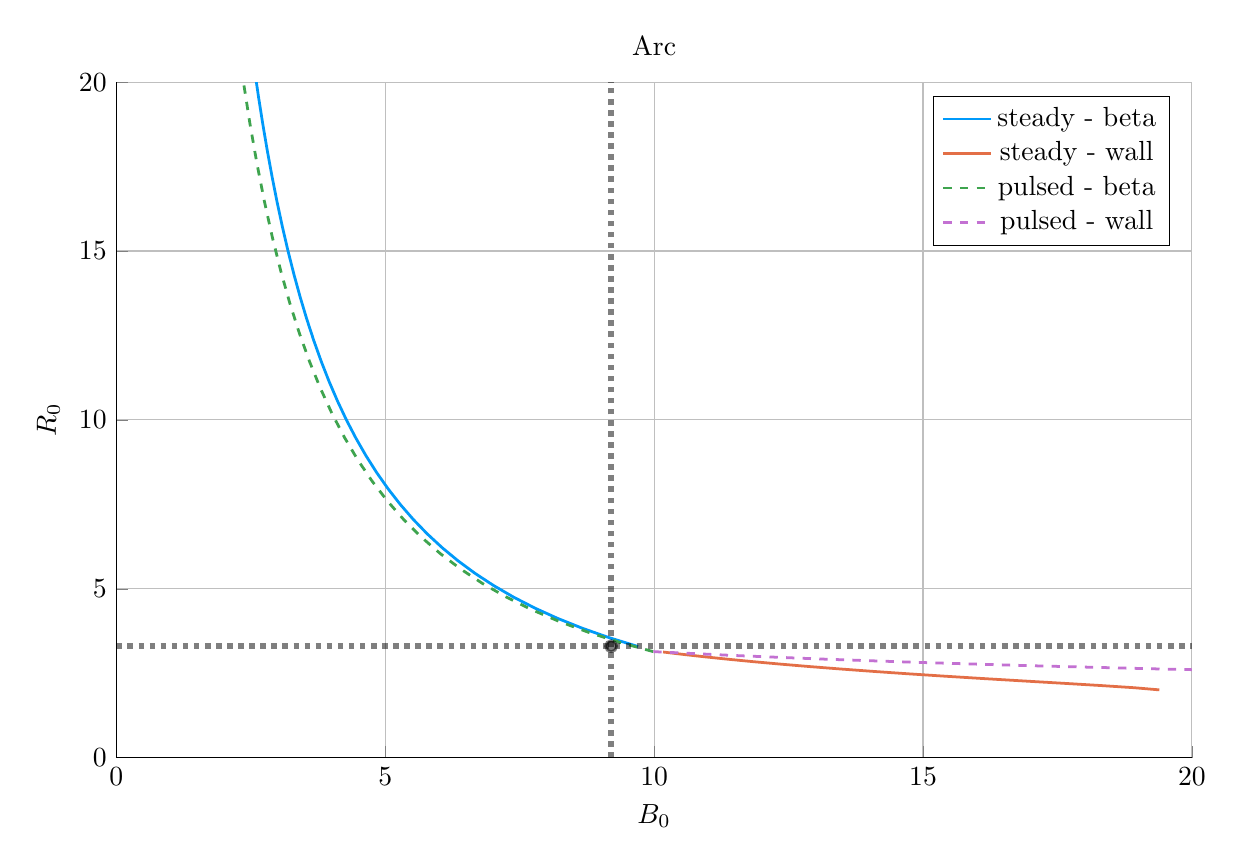
\begin{tikzpicture}[]
\begin{axis}[height = {101.6mm}, ylabel = {$R_0$}, title = {Arc}, xmin = {0.0}, xmax = {20.0}, ymax = {20.0}, xlabel = {$B_0$}, {unbounded coords=jump, scaled x ticks = false, xticklabel style={rotate = 0}, xmajorgrids = true, xtick = {0.0,5.0,10.0,15.0,20.0}, xticklabels = {0,5,10,15,20}, xtick align = inside, axis lines* = left, scaled y ticks = false, yticklabel style={rotate = 0}, ymajorgrids = true, ytick = {0.0,5.0,10.0,15.0,20.0}, yticklabels = {0,5,10,15,20}, ytick align = inside, axis lines* = left,     xshift = 0.0mm,
    yshift = 0.0mm,
    axis background/.style={fill={rgb,1:red,1.00000000;green,1.00000000;blue,1.00000000}}
}, ymin = {0.0}, width = {152.4mm}]\addplot+ [color = {rgb,1:red,0.00000000;green,0.60560316;blue,0.97868012},
draw opacity=1.0,
line width=1,
solid,mark = none,
mark size = 2.0,
mark options = {
    color = {rgb,1:red,0.00000000;green,0.00000000;blue,0.00000000}, draw opacity = 1.0,
    fill = {rgb,1:red,0.00000000;green,0.60560316;blue,0.97868012}, fill opacity = 1.0,
    line width = 1,
    rotate = 0,
    solid
}]coordinates {
(9.701206080853105, 3.2904233285656006)
(9.162315904693079, 3.553631706046861)
(8.664301107137337, 3.8315748016260343)
(8.203576462497304, 4.124583886864978)
(7.776718537485166, 4.433072975674755)
(7.380720231870917, 4.75741949036414)
(7.012886014999712, 5.097987291342331)
(6.670795005901889, 5.4551257000070565)
(6.352268997292712, 5.829168567645448)
(6.055344682097163, 6.220433393277178)
(5.778249464564785, 6.629220493040615)
(5.519380338856715, 7.05581222339423)
(5.2772854007125325, 7.500472260074458)
(5.050647625972996, 7.963444934423652)
(4.838270606140816, 8.444954628380609)
(4.639065978019038, 8.94520522910952)
(4.4520423235376105, 9.464379643936518)
(4.276295348572609, 10.002639375969222)
(4.110999177018484, 10.56012416048812)
(3.9553986195015125, 11.136951661929974)
(3.8088022956698633, 11.733217231026282)
(3.6705765055641186, 12.34899372141899)
(3.54013975965751, 12.984331364849716)
(3.4169578891619192, 13.639257703809928)
(3.30053966845824, 14.313777580345645)
(3.1904328903033052, 15.007873179535935)
(3.086220842019516, 15.721504126002731)
(2.9875191373772063, 16.45460763166718)
(2.8939728644914635, 17.207098692842226)
(2.8052540149097247, 17.97887033463821)
(2.7210591632720242, 18.7697939005645)
(2.6411073705789065, 19.579719385129263)
(2.565138287279709, 20.40847580717446)
(2.492910435164382, 21.255871621630877)
(2.4241996494611984, 22.12169516733927)
(2.3587976646588236, 23.0057151485579)
(2.296510829425685, 23.907681147764652)
(2.237158937627476, 24.827324167354146)
(2.180574163874242, 25.764357197843207)
(2.126600093288366, 26.71847581021091)
(2.075090836295778, 27.689358770027713)
(2.0259102202234582, 28.676668671060817)
(1.978931050353818, 29.68005258608471)
(1.9340344338545452, 30.69914273267572)
(1.8911091606836798, 31.733557151818793)
(1.8500511361739687, 32.78290039722107)
(1.8107628605384507, 33.846764233283025)
(1.773152951016952, 34.92472833975579)
(1.7371357028100902, 36.01636102117257)
(1.7026306853269466, 37.121219919229354)
(1.6695623706125668, 38.23885272635799)
(1.6378597911249178, 39.368797898817405)
(1.607456224302725, 40.51058536770822)
(1.5782889016090462, 41.663737246396295)
(1.5502987399539199, 42.82776853291479)
(1.5234300935954943, 44.00218780599217)
(1.4976305247952577, 45.18649791343829)
(1.4728505916614916, 46.38019665170201)
(1.4490436517578602, 47.58277743549339)
(1.4261656801829077, 48.79372995643627)
};
\addlegendentry{steady - beta}
\addplot+ [color = {rgb,1:red,0.88887350;green,0.43564919;blue,0.27812294},
draw opacity=1.0,
line width=1,
solid,mark = none,
mark size = 2.0,
mark options = {
    color = {rgb,1:red,0.00000000;green,0.00000000;blue,0.00000000}, draw opacity = 1.0,
    fill = {rgb,1:red,0.88887350;green,0.43564919;blue,0.27812294}, fill opacity = 1.0,
    line width = 1,
    rotate = 0,
    solid
}]coordinates {
(19.394007482712425, 2.006855814841082)
(18.932196567189358, 2.070220226465634)
(18.296989378345195, 2.1362327099649083)
(17.587029315408756, 2.2039322514902886)
(16.847882407994106, 2.272885741349308)
(16.111374502564406, 2.3427307443133163)
(15.396027314547156, 2.4132115621474344)
(14.710952688793137, 2.484165095168367)
(14.06168447794857, 2.555449485048069)
(13.450465418483889, 2.6269568263788754)
(12.877644538645335, 2.6986005527245354)
(12.342394470642008, 2.7703103261458715)
(11.843182246608265, 2.8420284550528074)
(11.376441269625893, 2.9137564749008216)
(10.944966372727551, 2.985307257194073)
(10.541663878705513, 3.056795384934831)
(10.165908182236457, 3.128148092221394)
};
\addlegendentry{steady - wall}
\addplot+ [color = {rgb,1:red,0.24222430;green,0.64327509;blue,0.30444865},
draw opacity=1.0,
line width=1,
dashed,mark = none,
mark size = 2.0,
mark options = {
    color = {rgb,1:red,0.00000000;green,0.00000000;blue,0.00000000}, draw opacity = 1.0,
    fill = {rgb,1:red,0.24222430;green,0.64327509;blue,0.30444865}, fill opacity = 1.0,
    line width = 1,
    rotate = 0,
    solid
}]coordinates {
(9.980483622051658, 3.1402982942956537)
(9.392786903460065, 3.3984668375583613)
(8.79273598103983, 3.7029994270206985)
(8.23820290909994, 4.029752381934837)
(7.725182218401588, 4.380005330007902)
(7.250078106370205, 4.755088191072525)
(6.80965553466646, 5.15638156809462)
(6.400998063035608, 5.585317075247801)
(6.0214713600430425, 6.043377623224966)
(5.668691517461799, 6.532097691007738)
(5.340497445229901, 7.053063624618788)
(5.034926745580058, 7.607914017422467)
(4.750194564008521, 8.198340243900201)
(4.484674995755211, 8.826087240213646)
(4.236884692979903, 9.49295465115087)
(4.00546837264544, 10.200798495308337)
(3.7891859704718387, 10.951533539957822)
(3.5869012239550364, 11.747136625739826)
(3.3975714987448393, 12.589651241396528)
(3.2202386987489797, 13.481193723261853)
(3.0540211220494466, 14.423961547290066)
(2.8981061427709687, 15.420244298711943)
(2.7517436139566023, 16.472438053930638)
(2.6142398986781377, 17.58306410230943)
(2.4849524463010138, 18.754793188384546)
(2.363284838174807, 19.990476791576892)
(2.248682232019848, 21.293187416028662)
(2.140627136740878, 22.666270490916787)
(2.038635448877246, 24.113411362836906)
(1.9422526775794744, 25.638722123308433)
(1.8510502754751532, 27.246854857488287)
(1.7646219756564088, 28.94315065234289)
(1.6825800061969869, 30.73383791051506)
(1.6045510059627948, 32.62630011975996)
(1.53017138625397, 34.629443897654504)
(1.4590817483192686, 36.754215952550474)
(1.3909197311384796, 39.01434852880224)
(1.3253102336217724, 41.42746903285954)
(1.261851128383913, 44.01681696754988)
(1.20009089049112, 46.81403058684408)
(1.1394908096975784, 49.863950342519615)
};
\addlegendentry{pulsed - beta}
\addplot+ [color = {rgb,1:red,0.76444018;green,0.44411178;blue,0.82429754},
draw opacity=1.0,
line width=1,
dashed,mark = none,
mark size = 2.0,
mark options = {
    color = {rgb,1:red,0.00000000;green,0.00000000;blue,0.00000000}, draw opacity = 1.0,
    fill = {rgb,1:red,0.76444018;green,0.44411178;blue,0.82429754}, fill opacity = 1.0,
    line width = 1,
    rotate = 0,
    solid
}]coordinates {
(29.27715761652869, 2.3448804182939873)
(25.4410619834368, 2.4377937236066716)
(22.158819835998365, 2.5322208586485804)
(19.342453256965573, 2.628163744265164)
(16.919364280634177, 2.7256238396687067)
(14.829378672669455, 2.8246020951898183)
(13.022412368922526, 2.9250989082568273)
(11.456617692058645, 3.0271140820266207)
(10.096901921254785, 3.1306467862637533)
(9.980483622051658, 3.1402982942956537)
};
\addlegendentry{pulsed - wall}
\addplot+ [color = {rgb,1:red,0.00000000;green,0.00000000;blue,0.00000000},
draw opacity=0.5,
line width=2,
dotted,mark = none,
mark size = 2.0,
mark options = {
    color = {rgb,1:red,0.00000000;green,0.00000000;blue,0.00000000}, draw opacity = 0.5,
    fill = {rgb,1:red,0.00000000;green,0.00000000;blue,0.00000000}, fill opacity = 0.5,
    line width = 1,
    rotate = 0,
    solid
},forget plot]coordinates {
(0.0, 3.3)
(20.0, 3.3)
};
\addplot+ [color = {rgb,1:red,0.00000000;green,0.00000000;blue,0.00000000},
draw opacity=0.5,
line width=2,
dotted,mark = none,
mark size = 2.0,
mark options = {
    color = {rgb,1:red,0.00000000;green,0.00000000;blue,0.00000000}, draw opacity = 0.5,
    fill = {rgb,1:red,0.00000000;green,0.00000000;blue,0.00000000}, fill opacity = 0.5,
    line width = 1,
    rotate = 0,
    solid
},forget plot]coordinates {
(9.2, 0.0)
(9.2, 20.0)
};
\addplot+[draw=none, color = {rgb,1:red,0.00000000;green,0.00000000;blue,0.00000000},
draw opacity=0.5,
line width=0,
solid,mark = *,
mark size = 2.0,
mark options = {
    color = {rgb,1:red,0.00000000;green,0.00000000;blue,0.00000000}, draw opacity = 0.5,
    fill = {rgb,1:red,0.00000000;green,0.00000000;blue,0.00000000}, fill opacity = 0.5,
    line width = 1,
    rotate = 0,
    solid
},forget plot] coordinates {
(9.2, 3.3)
};
\end{axis}

\end{tikzpicture}

    \end{adjustbox}
        \caption{$R_0$ vs $B_0$}
    \end{subfigure}
    \hfill
    \begin{subfigure}[t]{0.45\textwidth}
        \centering
    \begin{adjustbox}{width=\textwidth}
      \Large
      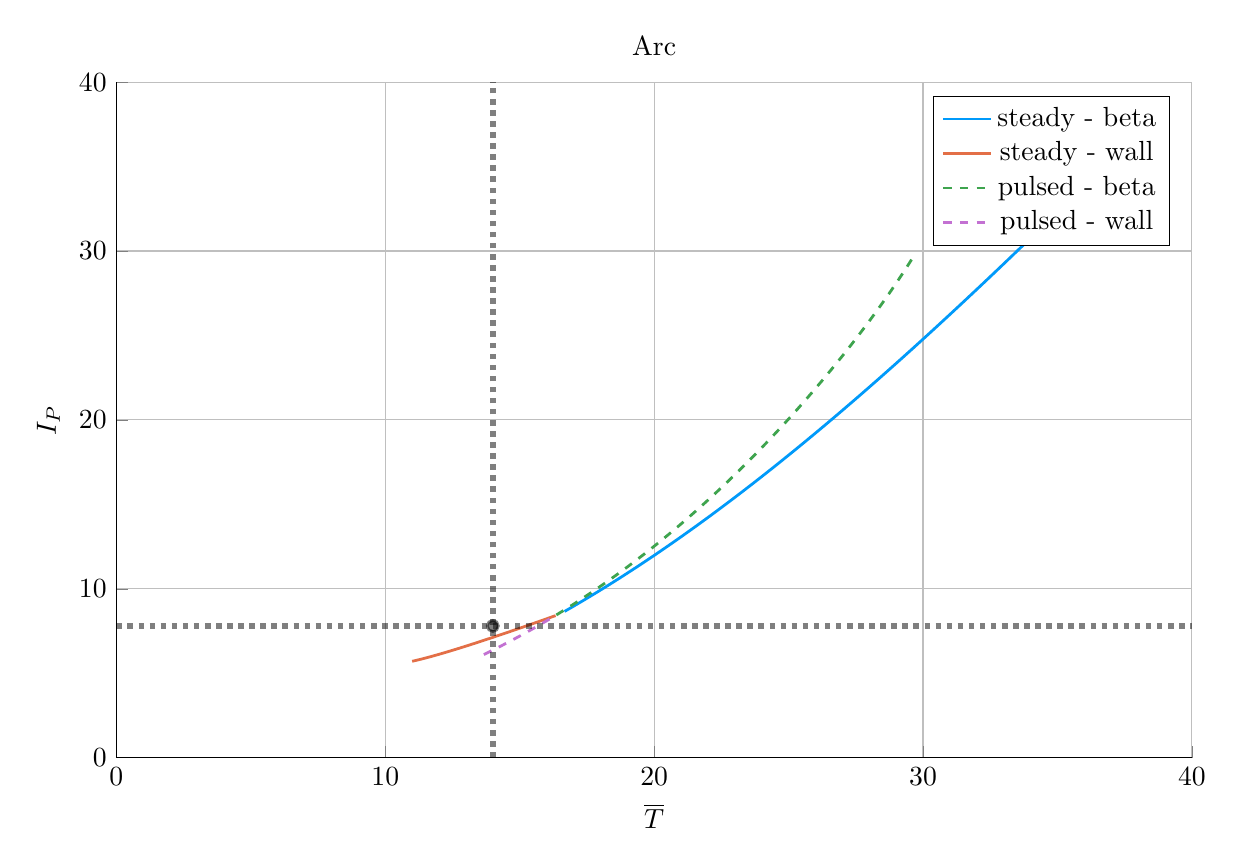
\begin{tikzpicture}[]
\begin{axis}[height = {101.6mm}, ylabel = {$I_P$}, title = {Arc}, xmin = {0.0}, xmax = {40.0}, ymax = {40.0}, xlabel = {$\overline T$}, {unbounded coords=jump, scaled x ticks = false, xticklabel style={rotate = 0}, xmajorgrids = true, xtick = {0.0,10.0,20.0,30.0,40.0}, xticklabels = {0,10,20,30,40}, xtick align = inside, axis lines* = left, scaled y ticks = false, yticklabel style={rotate = 0}, ymajorgrids = true, ytick = {0.0,10.0,20.0,30.0,40.0}, yticklabels = {0,10,20,30,40}, ytick align = inside, axis lines* = left,     xshift = 0.0mm,
    yshift = 0.0mm,
    axis background/.style={fill={rgb,1:red,1.00000000;green,1.00000000;blue,1.00000000}}
}, ymin = {0.0}, width = {152.4mm}]\addplot+ [color = {rgb,1:red,0.00000000;green,0.60560316;blue,0.97868012},
draw opacity=1.0,
line width=1,
solid,mark = none,
mark size = 2.0,
mark options = {
    color = {rgb,1:red,0.00000000;green,0.00000000;blue,0.00000000}, draw opacity = 1.0,
    fill = {rgb,1:red,0.00000000;green,0.60560316;blue,0.97868012}, fill opacity = 1.0,
    line width = 1,
    rotate = 0,
    solid
}]coordinates {
(16.666666666666668, 8.658343870907427)
(17.0, 8.964855141636448)
(17.333333333333332, 9.277118721367206)
(17.666666666666668, 9.595036914426)
(18.0, 9.918585776352757)
(18.333333333333332, 10.247718935951552)
(18.666666666666668, 10.582387319200262)
(19.0, 10.922539274323045)
(19.333333333333332, 11.26812069483817)
(19.666666666666668, 11.61907514056121)
(20.0, 11.975343956529299)
(20.333333333333332, 12.336866389803589)
(20.666666666666668, 12.703579704100664)
(21.0, 13.07541929220057)
(21.333333333333332, 13.452318786079019)
(21.666666666666668, 13.834210164711733)
(22.0, 14.221023859501257)
(22.333333333333332, 14.61268885728139)
(22.666666666666668, 15.009132800857182)
(23.0, 15.410282087044596)
(23.333333333333332, 15.816061962178953)
(23.666666666666668, 16.226396615066992)
(24.0, 16.64120926736311)
(24.333333333333332, 17.060422261356294)
(24.666666666666668, 17.483957145159597)
(25.0, 17.91173475530017)
(25.333333333333332, 18.343675296712746)
(25.666666666666668, 18.77969842014449)
(26.0, 19.2197232969848)
(26.333333333333332, 19.663668691537165)
(26.666666666666668, 20.11145303075519)
(27.0, 20.562994471468567)
(27.333333333333332, 21.018210965128485)
(27.666666666666668, 21.477020320105293)
(28.0, 21.939340261574117)
(28.333333333333332, 22.405088489026962)
(28.666666666666668, 22.874182731452617)
(29.0, 23.34654080022686)
(29.333333333333332, 23.82208063975841)
(29.666666666666668, 24.300720375936947)
(30.0, 24.782378362431352)
(30.333333333333332, 25.26697322488704)
(30.666666666666668, 25.754423903072542)
(31.0, 26.244649691026318)
(31.333333333333332, 26.737570275254438)
(31.666666666666668, 27.233105771031717)
(32.0, 27.731176756857092)
(32.333333333333336, 28.23170430711659)
(32.666666666666664, 28.734610023004112)
(33.0, 29.23981606175298)
(33.333333333333336, 29.747245164229085)
(33.666666666666664, 30.256820680936514)
(34.0, 30.768466596486252)
(34.333333333333336, 31.282107552577845)
(34.666666666666664, 31.797668869543177)
(35.0, 32.31507656650066)
(35.333333333333336, 32.83425738016771)
(35.666666666666664, 33.35513878237846)
(36.0, 33.87764899635294)
(36.333333333333336, 34.40171701176134)
};
\addlegendentry{steady - beta}
\addplot+ [color = {rgb,1:red,0.88887350;green,0.43564919;blue,0.27812294},
draw opacity=1.0,
line width=1,
solid,mark = none,
mark size = 2.0,
mark options = {
    color = {rgb,1:red,0.00000000;green,0.00000000;blue,0.00000000}, draw opacity = 1.0,
    fill = {rgb,1:red,0.88887350;green,0.43564919;blue,0.27812294}, fill opacity = 1.0,
    line width = 1,
    rotate = 0,
    solid
}]coordinates {
(11.0, 5.705363947896813)
(11.333333333333334, 5.831631927327359)
(11.666666666666666, 5.971358416795512)
(12.0, 6.120248050030096)
(12.333333333333334, 6.27635241161913)
(12.666666666666666, 6.438084943966173)
(13.0, 6.6043437111573775)
(13.333333333333334, 6.774432932493379)
(13.666666666666666, 6.9477586358526295)
(14.0, 7.123875039246037)
(14.333333333333334, 7.302428845502918)
(14.666666666666666, 7.483135839919747)
(15.0, 7.66576464137543)
(15.333333333333334, 7.850323804140159)
(15.666666666666666, 8.036059275223955)
(16.0, 8.223435700494395)
(16.333333333333332, 8.412159667095638)
};
\addlegendentry{steady - wall}
\addplot+ [color = {rgb,1:red,0.24222430;green,0.64327509;blue,0.30444865},
draw opacity=1.0,
line width=1,
dashed,mark = none,
mark size = 2.0,
mark options = {
    color = {rgb,1:red,0.00000000;green,0.00000000;blue,0.00000000}, draw opacity = 1.0,
    fill = {rgb,1:red,0.24222430;green,0.64327509;blue,0.30444865}, fill opacity = 1.0,
    line width = 1,
    rotate = 0,
    solid
}]coordinates {
(16.364160609330686, 8.45211123232532)
(16.666666666666668, 8.749174237506722)
(17.0, 9.084875445329175)
(17.333333333333332, 9.429466194729264)
(17.666666666666668, 9.783065958753857)
(18.0, 10.145791398086809)
(18.333333333333332, 10.517756265001724)
(18.666666666666668, 10.899071333792335)
(19.0, 11.28984436597908)
(19.333333333333332, 11.690180120182706)
(19.666666666666668, 12.100180418434789)
(20.0, 12.519944282916168)
(20.333333333333332, 12.949568159742276)
(20.666666666666668, 13.389146249526421)
(21.0, 13.838770968145022)
(21.333333333333332, 14.298533565526986)
(21.666666666666668, 14.768524935556082)
(22.0, 15.2488366565296)
(22.333333333333332, 15.739562309352701)
(22.666666666666668, 16.240799130174846)
(23.0, 16.752650066058415)
(23.333333333333332, 17.27522631730515)
(23.666666666666668, 17.808650469386293)
(24.0, 18.353060342640163)
(24.333333333333332, 18.908613721362002)
(24.666666666666668, 19.475494169025602)
(25.0, 20.053918198206937)
(25.333333333333332, 20.644144149900036)
(25.666666666666668, 21.246483258877372)
(26.0, 21.861313557471373)
(26.333333333333332, 22.48909752802998)
(26.666666666666668, 23.130404800381292)
(27.0, 23.785941781633092)
(27.333333333333332, 24.456591033172632)
(27.666666666666668, 25.143464707502787)
(28.0, 25.84797885666414)
(28.333333333333332, 26.571959755666764)
(28.666666666666668, 27.3178012356156)
(29.0, 28.088707029156687)
(29.333333333333332, 28.889082725820668)
(29.666666666666668, 29.725209471035893)
};
\addlegendentry{pulsed - beta}
\addplot+ [color = {rgb,1:red,0.76444018;green,0.44411178;blue,0.82429754},
draw opacity=1.0,
line width=1,
dashed,mark = none,
mark size = 2.0,
mark options = {
    color = {rgb,1:red,0.00000000;green,0.00000000;blue,0.00000000}, draw opacity = 1.0,
    fill = {rgb,1:red,0.76444018;green,0.44411178;blue,0.82429754}, fill opacity = 1.0,
    line width = 1,
    rotate = 0,
    solid
}]coordinates {
(13.666666666666666, 6.106956435644008)
(14.0, 6.368429153074452)
(14.333333333333334, 6.637611037727747)
(14.666666666666666, 6.914640849606676)
(15.0, 7.199655680909235)
(15.333333333333334, 7.492790823032018)
(15.666666666666666, 7.794179619860046)
(16.0, 8.103953307930404)
(16.333333333333332, 8.422240844292133)
(16.364160609330686, 8.45211123232532)
};
\addlegendentry{pulsed - wall}
\addplot+ [color = {rgb,1:red,0.00000000;green,0.00000000;blue,0.00000000},
draw opacity=0.5,
line width=2,
dotted,mark = none,
mark size = 2.0,
mark options = {
    color = {rgb,1:red,0.00000000;green,0.00000000;blue,0.00000000}, draw opacity = 0.5,
    fill = {rgb,1:red,0.00000000;green,0.00000000;blue,0.00000000}, fill opacity = 0.5,
    line width = 1,
    rotate = 0,
    solid
},forget plot]coordinates {
(0.0, 7.8)
(40.0, 7.8)
};
\addplot+ [color = {rgb,1:red,0.00000000;green,0.00000000;blue,0.00000000},
draw opacity=0.5,
line width=2,
dotted,mark = none,
mark size = 2.0,
mark options = {
    color = {rgb,1:red,0.00000000;green,0.00000000;blue,0.00000000}, draw opacity = 0.5,
    fill = {rgb,1:red,0.00000000;green,0.00000000;blue,0.00000000}, fill opacity = 0.5,
    line width = 1,
    rotate = 0,
    solid
},forget plot]coordinates {
(14.0, 0.0)
(14.0, 40.0)
};
\addplot+[draw=none, color = {rgb,1:red,0.00000000;green,0.00000000;blue,0.00000000},
draw opacity=0.5,
line width=0,
solid,mark = *,
mark size = 2.0,
mark options = {
    color = {rgb,1:red,0.00000000;green,0.00000000;blue,0.00000000}, draw opacity = 0.5,
    fill = {rgb,1:red,0.00000000;green,0.00000000;blue,0.00000000}, fill opacity = 0.5,
    line width = 1,
    rotate = 0,
    solid
},forget plot] coordinates {
(14.0, 7.8)
};
\end{axis}

\end{tikzpicture}

    \end{adjustbox}
        \caption{$I_P$ vs $\overline T$}
    \end{subfigure}
    \hfill \hfill ~\\ ~\\ ~\\
    \caption{Arc Model Comparison} ~\\
\end{figure*}

\begin{table}[h!]
\centering  
\caption{Arc Variables}
\hfill
\begin{subtable}[t]{0.4\textwidth}
\centering  
\caption{Input Variables} ~\\
\begin{tabular}{ c|c } 

Input            & Value           \\
\hline
$H$              & 1.8             \\
$Q$              & 13.6            \\
$N_{G}$          & 0.67            \\
$\epsilon$       & 0.3333          \\
$\kappa_{95}$    & 1.84            \\
$\delta_{95}$    & 0.333           \\
$\nu_{n}$        & 0.385           \\
$\nu_{T}$        & 0.929           \\
$l_{i}$          & 0.67            \\
$A$              & 2.5             \\
$Z_{eff}$        & 1.2             \\
$f_{D}$          & 0.9             \\
$\tau_{FT}$      & 1.6e9           \\
$B_{CS}$         & 12.77           \\

\end{tabular}
\end{subtable}
\hfill
\begin{subtable}[t]{0.5\textwidth}
\centering  
\caption{Output Variables} ~\\
\begin{tabular}{ c|c|c } 

Output           & Original         & Fussy.jl        \\
\hline
$R_{0}$          & 3.3              & 3.382           \\
$B_{0}$          & 9.2              & 9.505           \\
$I_{P}$          & 7.8              & 8.766           \\
$\overline n$    & 1.3              & 1.291           \\
$\overline T$    & 14.0             & 16.78           \\
$\beta_{N}$       & 0.0259           & 0.0259          \\
$q_{95}$         & 7.2              & 6.127           \\
$P_{W}$          & 2.5              & 2.215           \\
$f_{BS}$         & 0.63             & 0.5588          \\
$f_{CD}$         & 0.37             & 0.4412          \\
$f_{IN}$         & -              & -             \\
$\volume$         & 141.0            & 157.4           \\
$P_{F}$          & 525.0            & 725.9           \\
$\eta_{CD}$      & 0.321            & 0.3164          \\

\end{tabular}
\end{subtable}
\hfill
\hfill
\end{table}

\newpage

\subsection{Contrasting with the Aries Act Studies}

\newpage 

\subsubsection{Act I -- Advanced Physics and Engineering}

\begin{figure*}[h!]
    \centering
    \hfill 
    \begin{subfigure}[t]{0.45\textwidth}
        \centering
    \begin{adjustbox}{width=\textwidth}
      \Large
      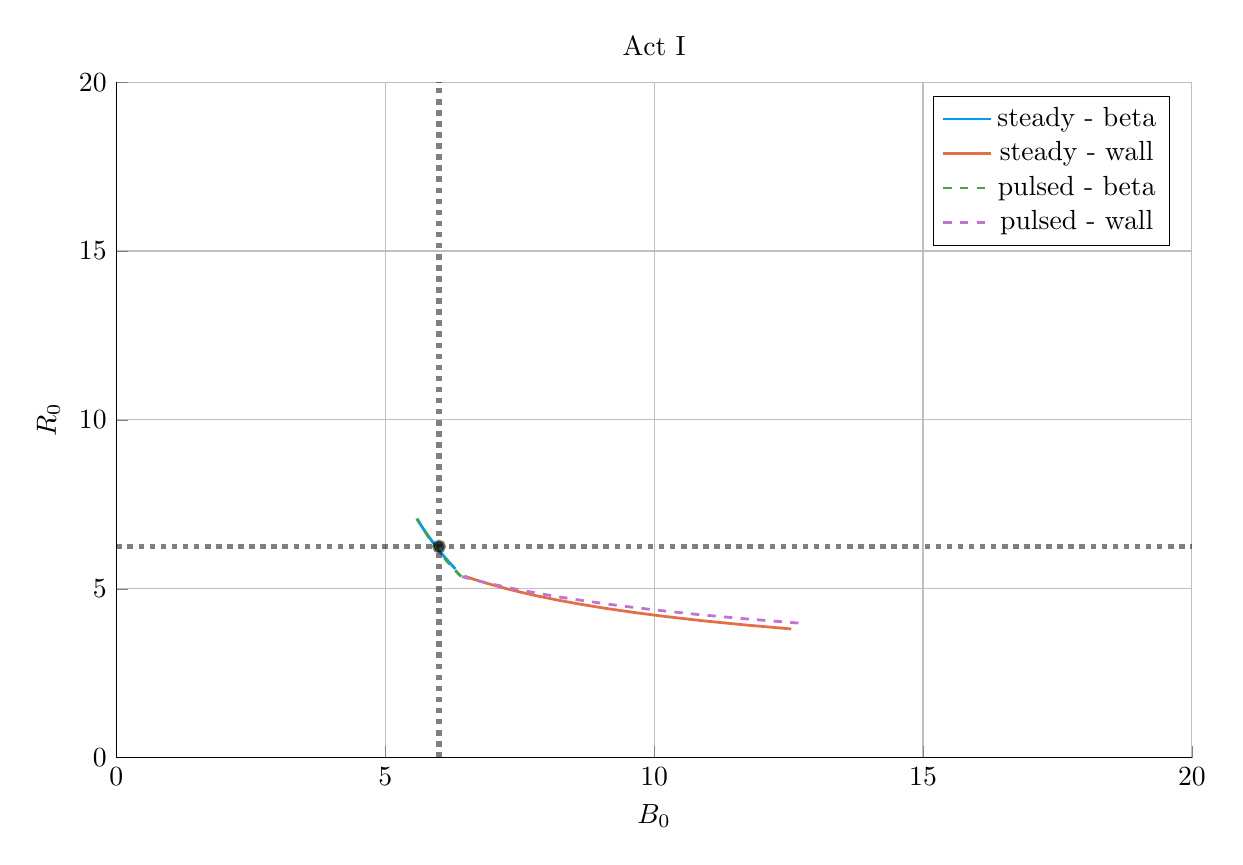
\begin{tikzpicture}[]
\begin{axis}[height = {101.6mm}, ylabel = {$R_0$}, title = {Act I}, xmin = {0.0}, xmax = {20.0}, ymax = {20.0}, xlabel = {$B_0$}, {unbounded coords=jump, scaled x ticks = false, xticklabel style={rotate = 0}, xmajorgrids = true, xtick = {0.0,5.0,10.0,15.0,20.0}, xticklabels = {0,5,10,15,20}, xtick align = inside, axis lines* = left, scaled y ticks = false, yticklabel style={rotate = 0}, ymajorgrids = true, ytick = {0.0,5.0,10.0,15.0,20.0}, yticklabels = {0,5,10,15,20}, ytick align = inside, axis lines* = left,     xshift = 0.0mm,
    yshift = 0.0mm,
    axis background/.style={fill={rgb,1:red,1.00000000;green,1.00000000;blue,1.00000000}}
}, ymin = {0.0}, width = {152.4mm}]\addplot+ [color = {rgb,1:red,0.00000000;green,0.60560316;blue,0.97868012},
draw opacity=1.0,
line width=1,
solid,mark = none,
mark size = 2.0,
mark options = {
    color = {rgb,1:red,0.00000000;green,0.00000000;blue,0.00000000}, draw opacity = 1.0,
    fill = {rgb,1:red,0.00000000;green,0.60560316;blue,0.97868012}, fill opacity = 1.0,
    line width = 1,
    rotate = 0,
    solid
}]coordinates {
(6.30336807958207, 5.587199391496101)
(6.162193069273141, 5.831838137107903)
(6.030717178404645, 6.078157823726375)
(5.908065509576601, 6.325994353145188)
(5.793464904530972, 6.57518910191267)
(5.686229631357383, 6.825588847053452)
(5.585749511271037, 7.077045564754442)
};
\addlegendentry{steady - beta}
\addplot+ [color = {rgb,1:red,0.88887350;green,0.43564919;blue,0.27812294},
draw opacity=1.0,
line width=1,
solid,mark = none,
mark size = 2.0,
mark options = {
    color = {rgb,1:red,0.00000000;green,0.00000000;blue,0.00000000}, draw opacity = 1.0,
    fill = {rgb,1:red,0.88887350;green,0.43564919;blue,0.27812294}, fill opacity = 1.0,
    line width = 1,
    rotate = 0,
    solid
}]coordinates {
(12.549536249695134, 3.8108352245940957)
(11.658754653696462, 3.934083270736017)
(10.883719833507003, 4.057046546594516)
(10.206258129789394, 4.179626810883221)
(9.611335769312953, 4.301750356443285)
(9.086446934250878, 4.423366229113912)
(8.62129895070743, 4.544434218016914)
(8.207216040989662, 4.6649335402400025)
(7.837119555085499, 4.78484200403474)
(7.505047858717157, 4.9041467319817595)
(7.20604322925957, 5.022835870779136)
(6.935884710193303, 5.1409045607718795)
(6.691016583192173, 5.258349129805506)
(6.468415485086983, 5.375167957409874)
};
\addlegendentry{steady - wall}
\addplot+ [color = {rgb,1:red,0.24222430;green,0.64327509;blue,0.30444865},
draw opacity=1.0,
line width=1,
dashed,mark = none,
mark size = 2.0,
mark options = {
    color = {rgb,1:red,0.00000000;green,0.00000000;blue,0.00000000}, draw opacity = 1.0,
    fill = {rgb,1:red,0.24222430;green,0.64327509;blue,0.30444865}, fill opacity = 1.0,
    line width = 1,
    rotate = 0,
    solid
}]coordinates {
(6.408263337806559, 5.366131328829866)
(6.408263337806564, 5.366131328829862)
(6.385466513301022, 5.402805883604879)
(6.245492502072912, 5.638974714472524)
(6.116010320461132, 5.875875066688821)
(5.9960421481916395, 6.113307727774442)
(5.884727159112828, 6.351082733498888)
(5.781304768121868, 6.589019058920955)
(5.685100648450046, 6.826944315253105)
(5.595515000321003, 7.064694456596427)
};
\addlegendentry{pulsed - beta}
\addplot+ [color = {rgb,1:red,0.76444018;green,0.44411178;blue,0.82429754},
draw opacity=1.0,
line width=1,
dashed,mark = none,
mark size = 2.0,
mark options = {
    color = {rgb,1:red,0.00000000;green,0.00000000;blue,0.00000000}, draw opacity = 1.0,
    fill = {rgb,1:red,0.76444018;green,0.44411178;blue,0.82429754}, fill opacity = 1.0,
    line width = 1,
    rotate = 0,
    solid
}]coordinates {
(12.684248532650473, 3.9847907768802657)
(11.66307871570063, 4.114684512780648)
(10.781888309639141, 4.244124103742294)
(10.016282491385791, 4.373086052625054)
(9.346943280276514, 4.501549309887817)
(8.758420158941194, 4.6294950281779785)
(8.238241792953433, 4.756906348757686)
(7.776255600865612, 4.883768212546736)
(7.364131118520045, 5.010067192354689)
(6.994982564641668, 5.135791343697217)
(6.66307916140573, 5.260930071474144)
(6.408263337806559, 5.366131328829866)
(6.408263337806564, 5.366131328829862)
};
\addlegendentry{pulsed - wall}
\addplot+ [color = {rgb,1:red,0.00000000;green,0.00000000;blue,0.00000000},
draw opacity=0.5,
line width=2,
dotted,mark = none,
mark size = 2.0,
mark options = {
    color = {rgb,1:red,0.00000000;green,0.00000000;blue,0.00000000}, draw opacity = 0.5,
    fill = {rgb,1:red,0.00000000;green,0.00000000;blue,0.00000000}, fill opacity = 0.5,
    line width = 1,
    rotate = 0,
    solid
},forget plot]coordinates {
(0.0, 6.25)
(20.0, 6.25)
};
\addplot+ [color = {rgb,1:red,0.00000000;green,0.00000000;blue,0.00000000},
draw opacity=0.5,
line width=2,
dotted,mark = none,
mark size = 2.0,
mark options = {
    color = {rgb,1:red,0.00000000;green,0.00000000;blue,0.00000000}, draw opacity = 0.5,
    fill = {rgb,1:red,0.00000000;green,0.00000000;blue,0.00000000}, fill opacity = 0.5,
    line width = 1,
    rotate = 0,
    solid
},forget plot]coordinates {
(6.0, 0.0)
(6.0, 20.0)
};
\addplot+[draw=none, color = {rgb,1:red,0.00000000;green,0.00000000;blue,0.00000000},
draw opacity=0.5,
line width=0,
solid,mark = *,
mark size = 2.0,
mark options = {
    color = {rgb,1:red,0.00000000;green,0.00000000;blue,0.00000000}, draw opacity = 0.5,
    fill = {rgb,1:red,0.00000000;green,0.00000000;blue,0.00000000}, fill opacity = 0.5,
    line width = 1,
    rotate = 0,
    solid
},forget plot] coordinates {
(6.0, 6.25)
};
\end{axis}

\end{tikzpicture}

    \end{adjustbox}
        \caption{$R_0$ vs $B_0$}
    \end{subfigure}
    \hfill
    \begin{subfigure}[t]{0.45\textwidth}
        \centering
    \begin{adjustbox}{width=\textwidth}
      \Large
      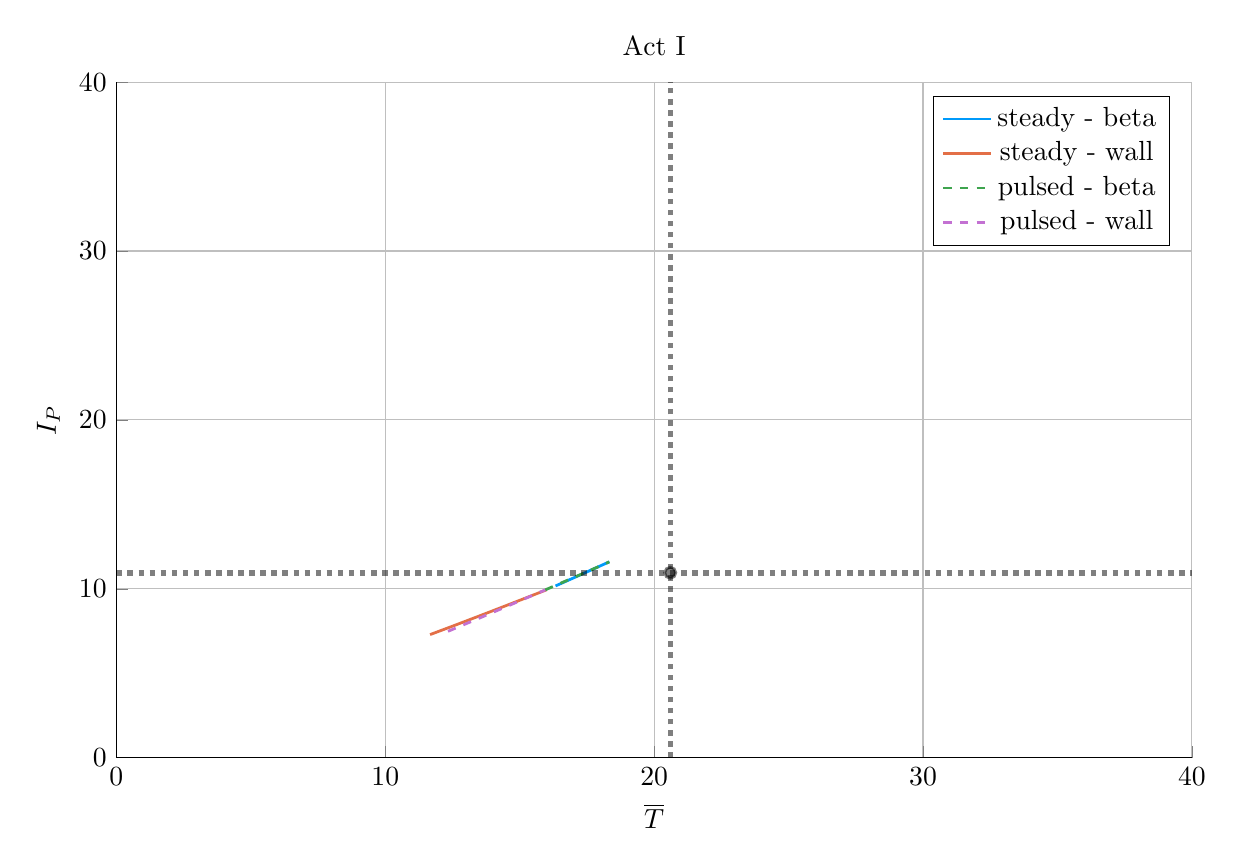
\begin{tikzpicture}[]
\begin{axis}[height = {101.6mm}, ylabel = {$I_P$}, title = {Act I}, xmin = {0.0}, xmax = {40.0}, ymax = {40.0}, xlabel = {$\overline T$}, {unbounded coords=jump, scaled x ticks = false, xticklabel style={rotate = 0}, xmajorgrids = true, xtick = {0.0,10.0,20.0,30.0,40.0}, xticklabels = {0,10,20,30,40}, xtick align = inside, axis lines* = left, scaled y ticks = false, yticklabel style={rotate = 0}, ymajorgrids = true, ytick = {0.0,10.0,20.0,30.0,40.0}, yticklabels = {0,10,20,30,40}, ytick align = inside, axis lines* = left,     xshift = 0.0mm,
    yshift = 0.0mm,
    axis background/.style={fill={rgb,1:red,1.00000000;green,1.00000000;blue,1.00000000}}
}, ymin = {0.0}, width = {152.4mm}]\addplot+ [color = {rgb,1:red,0.00000000;green,0.60560316;blue,0.97868012},
draw opacity=1.0,
line width=1,
solid,mark = none,
mark size = 2.0,
mark options = {
    color = {rgb,1:red,0.00000000;green,0.00000000;blue,0.00000000}, draw opacity = 1.0,
    fill = {rgb,1:red,0.00000000;green,0.60560316;blue,0.97868012}, fill opacity = 1.0,
    line width = 1,
    rotate = 0,
    solid
}]coordinates {
(16.333333333333332, 10.169194435531358)
(16.666666666666668, 10.405057509328124)
(17.0, 10.641905327194731)
(17.333333333333332, 10.87971637136811)
(17.666666666666668, 11.11846917050157)
(18.0, 11.358142407296011)
(18.333333333333332, 11.598714938197329)
};
\addlegendentry{steady - beta}
\addplot+ [color = {rgb,1:red,0.88887350;green,0.43564919;blue,0.27812294},
draw opacity=1.0,
line width=1,
solid,mark = none,
mark size = 2.0,
mark options = {
    color = {rgb,1:red,0.00000000;green,0.00000000;blue,0.00000000}, draw opacity = 1.0,
    fill = {rgb,1:red,0.88887350;green,0.43564919;blue,0.27812294}, fill opacity = 1.0,
    line width = 1,
    rotate = 0,
    solid
}]coordinates {
(11.666666666666666, 7.287903136887)
(12.0, 7.486025430610099)
(12.333333333333334, 7.685696663157812)
(12.666666666666666, 7.886645361110723)
(13.0, 8.08866940687473)
(13.333333333333334, 8.291629426976055)
(13.666666666666666, 8.495414075666067)
(14.0, 8.699964056113311)
(14.333333333333334, 8.905213556979005)
(14.666666666666666, 9.111120468746519)
(15.0, 9.31764336053339)
(15.333333333333334, 9.524758318501357)
(15.666666666666666, 9.732442959434447)
(16.0, 9.940679052729761)
};
\addlegendentry{steady - wall}
\addplot+ [color = {rgb,1:red,0.24222430;green,0.64327509;blue,0.30444865},
draw opacity=1.0,
line width=1,
dashed,mark = none,
mark size = 2.0,
mark options = {
    color = {rgb,1:red,0.00000000;green,0.00000000;blue,0.00000000}, draw opacity = 1.0,
    fill = {rgb,1:red,0.24222430;green,0.64327509;blue,0.30444865}, fill opacity = 1.0,
    line width = 1,
    rotate = 0,
    solid
}]coordinates {
(15.948125117373092, 9.933500150990564)
(15.9481251173731, 9.933500150990564)
(16.0, 9.969282740147014)
(16.333333333333332, 10.199548426407084)
(16.666666666666668, 10.430379144484162)
(17.0, 10.661750348679098)
(17.333333333333332, 10.893638132753678)
(17.666666666666668, 11.126019229767902)
(18.0, 11.358871009413285)
(18.333333333333332, 11.592171473618816)
};
\addlegendentry{pulsed - beta}
\addplot+ [color = {rgb,1:red,0.76444018;green,0.44411178;blue,0.82429754},
draw opacity=1.0,
line width=1,
dashed,mark = none,
mark size = 2.0,
mark options = {
    color = {rgb,1:red,0.00000000;green,0.00000000;blue,0.00000000}, draw opacity = 1.0,
    fill = {rgb,1:red,0.76444018;green,0.44411178;blue,0.82429754}, fill opacity = 1.0,
    line width = 1,
    rotate = 0,
    solid
}]coordinates {
(12.333333333333334, 7.481290856821823)
(12.666666666666666, 7.703549290655078)
(13.0, 7.92668121689452)
(13.333333333333334, 8.15065615613957)
(13.666666666666666, 8.375443966327172)
(14.0, 8.601014900773066)
(14.333333333333334, 8.82733966430566)
(14.666666666666666, 9.054389459546684)
(15.0, 9.282136024328327)
(15.333333333333334, 9.510551661584085)
(15.666666666666666, 9.73960926266661)
(15.948125117373092, 9.933500150990564)
(15.9481251173731, 9.933500150990564)
};
\addlegendentry{pulsed - wall}
\addplot+ [color = {rgb,1:red,0.00000000;green,0.00000000;blue,0.00000000},
draw opacity=0.5,
line width=2,
dotted,mark = none,
mark size = 2.0,
mark options = {
    color = {rgb,1:red,0.00000000;green,0.00000000;blue,0.00000000}, draw opacity = 0.5,
    fill = {rgb,1:red,0.00000000;green,0.00000000;blue,0.00000000}, fill opacity = 0.5,
    line width = 1,
    rotate = 0,
    solid
},forget plot]coordinates {
(0.0, 10.95)
(40.0, 10.95)
};
\addplot+ [color = {rgb,1:red,0.00000000;green,0.00000000;blue,0.00000000},
draw opacity=0.5,
line width=2,
dotted,mark = none,
mark size = 2.0,
mark options = {
    color = {rgb,1:red,0.00000000;green,0.00000000;blue,0.00000000}, draw opacity = 0.5,
    fill = {rgb,1:red,0.00000000;green,0.00000000;blue,0.00000000}, fill opacity = 0.5,
    line width = 1,
    rotate = 0,
    solid
},forget plot]coordinates {
(20.6, 0.0)
(20.6, 40.0)
};
\addplot+[draw=none, color = {rgb,1:red,0.00000000;green,0.00000000;blue,0.00000000},
draw opacity=0.5,
line width=0,
solid,mark = *,
mark size = 2.0,
mark options = {
    color = {rgb,1:red,0.00000000;green,0.00000000;blue,0.00000000}, draw opacity = 0.5,
    fill = {rgb,1:red,0.00000000;green,0.00000000;blue,0.00000000}, fill opacity = 0.5,
    line width = 1,
    rotate = 0,
    solid
},forget plot] coordinates {
(20.6, 10.95)
};
\end{axis}

\end{tikzpicture}

    \end{adjustbox}
        \caption{$I_P$ vs $\overline T$}
    \end{subfigure}
    \hfill \hfill ~\\ ~\\ ~\\
    \caption{Aries Act I Model Comparison} ~\\
\end{figure*}

\begin{table}[h!]
\centering  
\caption{Act I Variables}
\hfill
\begin{subtable}[t]{0.4\textwidth}
\centering  
\caption{Input Variables} ~\\
\begin{tabular}{ c|c } 

Input            & Value           \\
\hline
$H$              & 1.65            \\
$Q$              & 42.5            \\
$N_{G}$          & 1.0             \\
$\epsilon$       & 0.25            \\
$\kappa_{95}$    & 2.1             \\
$\delta_{95}$    & 0.4             \\
$\nu_{n}$        & 0.27            \\
$\nu_{T}$        & 1.15            \\
$l_{i}$          & 0.35906         \\
$A$              & 2.5             \\
$Z_{eff}$        & 2.11            \\
$f_{D}$          & 0.75            \\
$\tau_{FT}$      & 1.6e9           \\
$B_{CS}$         & 12.77           \\

\end{tabular}
\end{subtable}
\hfill
\begin{subtable}[t]{0.5\textwidth}
\centering  
\caption{Output Variables} ~\\
\begin{tabular}{ c|c|c } 

Output           & Original         & Fussy.jl        \\
\hline
$R_{0}$          & 6.25             & 6.226           \\
$B_{0}$          & 6.0              & 5.956           \\
$I_{P}$          & 10.95            & 10.78           \\
$\overline n$    & 1.3              & 1.288           \\
$\overline T$    & 20.6             & 17.2            \\
$\beta_{N}$       & 0.0427           & 0.0427          \\
$q_{95}$         & 4.5              & 3.993           \\
$P_{W}$          & 2.45             & 2.004           \\
$f_{BS}$         & 0.91             & 0.906           \\
$f_{CD}$         & 0.09             & 0.094           \\
$f_{IN}$         & -              & -             \\
$\volume$         & 582.0            & 621.4           \\
$P_{F}$          & 1813           & 1865          \\
$\eta_{CD}$      & 0.188            & 0.1853          \\

\end{tabular}
\end{subtable}
\hfill
\hfill
\end{table}

\newpage 

\subsubsection{Act II -- Conservative Physics and Engineering}

\begin{figure*}[h!]
    \centering
    \hfill 
    \begin{subfigure}[t]{0.45\textwidth}
        \centering
    \begin{adjustbox}{width=\textwidth}
      \Large
      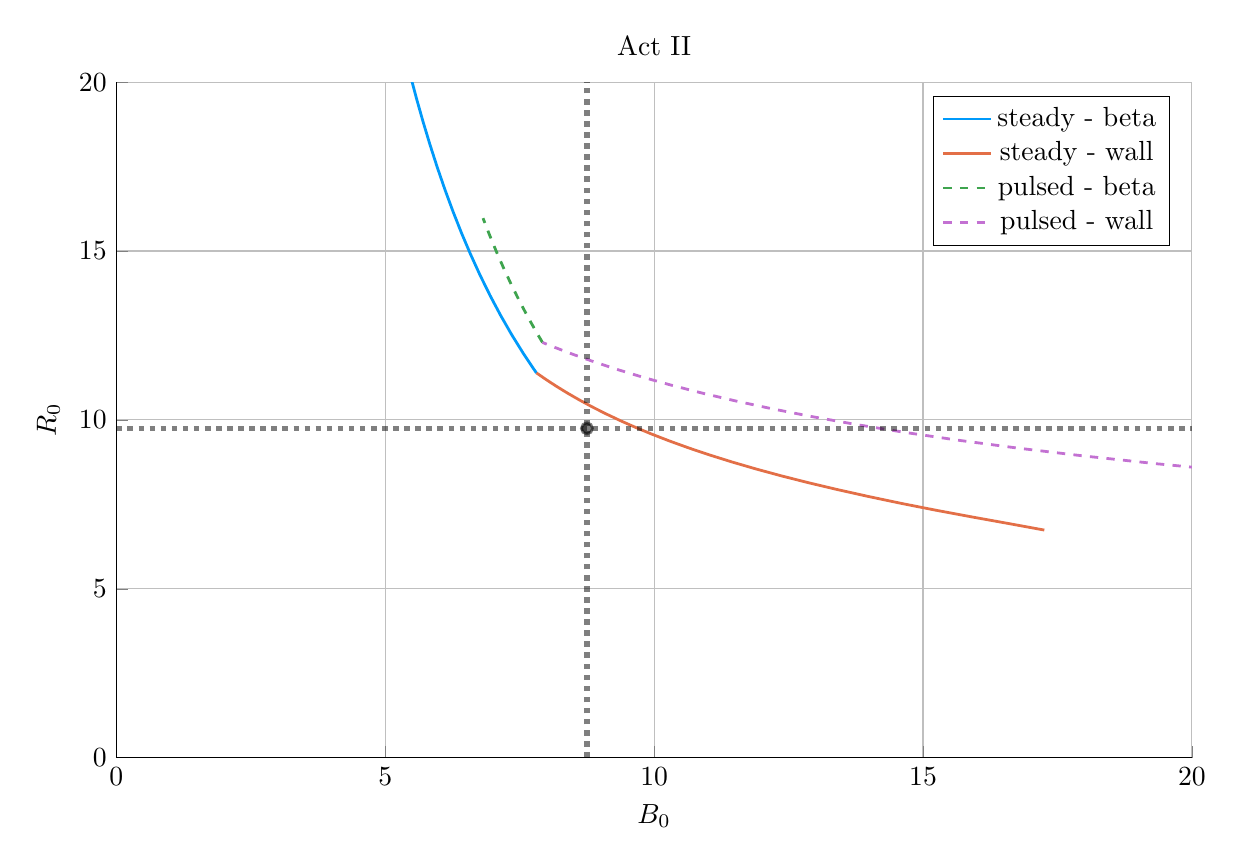
\begin{tikzpicture}[]
\begin{axis}[height = {101.6mm}, ylabel = {$R_0$}, title = {Act II}, xmin = {0.0}, xmax = {20.0}, ymax = {20.0}, xlabel = {$B_0$}, {unbounded coords=jump, scaled x ticks = false, xticklabel style={rotate = 0}, xmajorgrids = true, xtick = {0.0,5.0,10.0,15.0,20.0}, xticklabels = {0,5,10,15,20}, xtick align = inside, axis lines* = left, scaled y ticks = false, yticklabel style={rotate = 0}, ymajorgrids = true, ytick = {0.0,5.0,10.0,15.0,20.0}, yticklabels = {0,5,10,15,20}, ytick align = inside, axis lines* = left,     xshift = 0.0mm,
    yshift = 0.0mm,
    axis background/.style={fill={rgb,1:red,1.00000000;green,1.00000000;blue,1.00000000}}
}, ymin = {0.0}, width = {152.4mm}]\addplot+ [color = {rgb,1:red,0.00000000;green,0.60560316;blue,0.97868012},
draw opacity=1.0,
line width=1,
solid,mark = none,
mark size = 2.0,
mark options = {
    color = {rgb,1:red,0.00000000;green,0.00000000;blue,0.00000000}, draw opacity = 1.0,
    fill = {rgb,1:red,0.00000000;green,0.60560316;blue,0.97868012}, fill opacity = 1.0,
    line width = 1,
    rotate = 0,
    solid
}]coordinates {
(7.810935944285959, 11.389141268081966)
(7.57736049850867, 11.942634046586162)
(7.354864292609041, 12.51245847357923)
(7.145167234136329, 13.0943365692581)
(6.9473303865083675, 13.687993788149779)
(6.760499508614096, 14.293145886478186)
(6.583897990324067, 14.909495325365516)
(6.416817229618043, 15.536734694045393)
(6.258609820663305, 16.1745467994937)
(6.108683264880386, 16.82260538899235)
(5.966494431410919, 17.480575868750975)
(5.831544666176381, 18.148116014600475)
(5.703375459679132, 18.824876684423757)
(5.581564609582325, 19.510502502077443)
(5.465722802994068, 20.20463254880097)
(5.355490573482678, 20.906901035327614)
(5.25053558682053, 21.616937949657327)
(5.1505502068221745, 22.334369714080776)
(5.0552493196883175, 23.058819802110854)
};
\addlegendentry{steady - beta}
\addplot+ [color = {rgb,1:red,0.88887350;green,0.43564919;blue,0.27812294},
draw opacity=1.0,
line width=1,
solid,mark = none,
mark size = 2.0,
mark options = {
    color = {rgb,1:red,0.00000000;green,0.00000000;blue,0.00000000}, draw opacity = 1.0,
    fill = {rgb,1:red,0.88887350;green,0.43564919;blue,0.27812294}, fill opacity = 1.0,
    line width = 1,
    rotate = 0,
    solid
}]coordinates {
(17.25550839059296, 6.738604635617289)
(16.594334962335296, 6.931178286222189)
(15.9071755430688, 7.128187388035985)
(15.233983138507648, 7.327817939330552)
(14.594239858921854, 7.528927553154291)
(13.989673082630297, 7.7312042898700515)
(13.414782495717416, 7.934790159202381)
(12.872659546281994, 8.139273115071695)
(12.364365715508608, 8.344321605506495)
(11.889507953196574, 8.549679244077495)
(11.44685939646348, 8.755144058838903)
(11.034739998180656, 8.960554762148757)
(10.651252523287319, 9.165781242855727)
(10.294428800132035, 9.370717743724994)
(9.962319203963213, 9.57527782549947)
(9.653045819449929, 9.779390564591205)
(9.364832254395445, 9.982997628553138)
(9.096018465506306, 10.186050992034668)
(8.844373144802077, 10.388606525997883)
(8.61055754360846, 10.590345571972314)
(8.391192178573277, 10.791527736428888)
(8.18577947665566, 10.992035979756642)
(7.99323348423048, 11.1918525509058)
(7.812301489248497, 11.391007917726574)
};
\addlegendentry{steady - wall}
\addplot+ [color = {rgb,1:red,0.24222430;green,0.64327509;blue,0.30444865},
draw opacity=1.0,
line width=1,
dashed,mark = none,
mark size = 2.0,
mark options = {
    color = {rgb,1:red,0.00000000;green,0.00000000;blue,0.00000000}, draw opacity = 1.0,
    fill = {rgb,1:red,0.24222430;green,0.64327509;blue,0.30444865}, fill opacity = 1.0,
    line width = 1,
    rotate = 0,
    solid
}]coordinates {
(7.923668284887995, 12.293879059492616)
(7.923668284887995, 12.293879059492635)
(7.836759696043437, 12.52591633746021)
(7.6662731560983355, 13.00454403942661)
(7.50499428233835, 13.488375025456907)
(7.35232773269976, 13.977065733125242)
(7.207727224738343, 14.470269937628656)
(7.070690693175276, 14.967639476613451)
(6.940756001029682, 15.46882496625731)
(6.817497143644154, 15.973476480630131)
};
\addlegendentry{pulsed - beta}
\addplot+ [color = {rgb,1:red,0.76444018;green,0.44411178;blue,0.82429754},
draw opacity=1.0,
line width=1,
dashed,mark = none,
mark size = 2.0,
mark options = {
    color = {rgb,1:red,0.00000000;green,0.00000000;blue,0.00000000}, draw opacity = 1.0,
    fill = {rgb,1:red,0.76444018;green,0.44411178;blue,0.82429754}, fill opacity = 1.0,
    line width = 1,
    rotate = 0,
    solid
}]coordinates {
(22.56106430311702, 8.239911323116141)
(20.85607192394036, 8.471453471694678)
(19.335265246056654, 8.703260993170346)
(17.974121547130903, 8.935277031603567)
(16.751976718553127, 9.167446093344447)
(15.651329744019142, 9.399714010238458)
(14.65728744097675, 9.632027927077594)
(13.757118584462601, 9.864336290607328)
(12.939893642194303, 10.096588839007167)
(12.196191964860315, 10.328736591776112)
(11.517862472405039, 10.560731839999896)
(10.897827027335556, 10.792528137074703)
(10.329918077124672, 11.02408028901105)
(9.808743940706389, 11.255344346143936)
(9.329576544487265, 11.486277593626015)
(8.888257451278507, 11.716838542453242)
(8.481118883411932, 11.946986920205564)
(8.10491708701527, 12.17668366154026)
(7.923668284887995, 12.293879059492616)
(7.923668284887995, 12.293879059492635)
};
\addlegendentry{pulsed - wall}
\addplot+ [color = {rgb,1:red,0.00000000;green,0.00000000;blue,0.00000000},
draw opacity=0.5,
line width=2,
dotted,mark = none,
mark size = 2.0,
mark options = {
    color = {rgb,1:red,0.00000000;green,0.00000000;blue,0.00000000}, draw opacity = 0.5,
    fill = {rgb,1:red,0.00000000;green,0.00000000;blue,0.00000000}, fill opacity = 0.5,
    line width = 1,
    rotate = 0,
    solid
},forget plot]coordinates {
(0.0, 9.75)
(20.0, 9.75)
};
\addplot+ [color = {rgb,1:red,0.00000000;green,0.00000000;blue,0.00000000},
draw opacity=0.5,
line width=2,
dotted,mark = none,
mark size = 2.0,
mark options = {
    color = {rgb,1:red,0.00000000;green,0.00000000;blue,0.00000000}, draw opacity = 0.5,
    fill = {rgb,1:red,0.00000000;green,0.00000000;blue,0.00000000}, fill opacity = 0.5,
    line width = 1,
    rotate = 0,
    solid
},forget plot]coordinates {
(8.75, 0.0)
(8.75, 20.0)
};
\addplot+[draw=none, color = {rgb,1:red,0.00000000;green,0.00000000;blue,0.00000000},
draw opacity=0.5,
line width=0,
solid,mark = *,
mark size = 2.0,
mark options = {
    color = {rgb,1:red,0.00000000;green,0.00000000;blue,0.00000000}, draw opacity = 0.5,
    fill = {rgb,1:red,0.00000000;green,0.00000000;blue,0.00000000}, fill opacity = 0.5,
    line width = 1,
    rotate = 0,
    solid
},forget plot] coordinates {
(8.75, 9.75)
};
\end{axis}

\end{tikzpicture}

    \end{adjustbox}
        \caption{$R_0$ vs $B_0$}
    \end{subfigure}
    \hfill
    \begin{subfigure}[t]{0.45\textwidth}
        \centering
    \begin{adjustbox}{width=\textwidth}
      \Large
      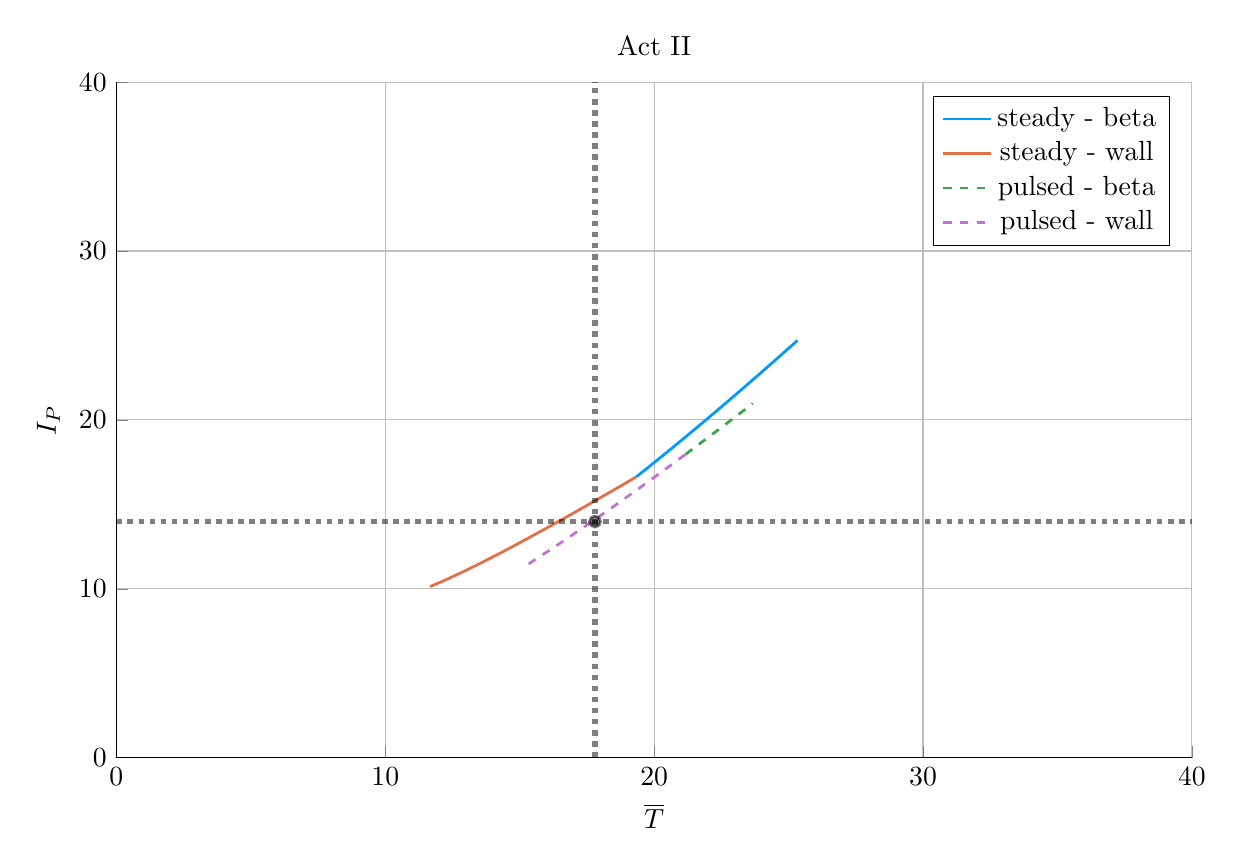
\begin{tikzpicture}[]
\begin{axis}[height = {101.6mm}, ylabel = {$I_P$}, title = {Act II}, xmin = {0.0}, xmax = {40.0}, ymax = {40.0}, xlabel = {$\overline T$}, {unbounded coords=jump, scaled x ticks = false, xticklabel style={rotate = 0}, xmajorgrids = true, xtick = {0.0,10.0,20.0,30.0,40.0}, xticklabels = {0,10,20,30,40}, xtick align = inside, axis lines* = left, scaled y ticks = false, yticklabel style={rotate = 0}, ymajorgrids = true, ytick = {0.0,10.0,20.0,30.0,40.0}, yticklabels = {0,10,20,30,40}, ytick align = inside, axis lines* = left,     xshift = 0.0mm,
    yshift = 0.0mm,
    axis background/.style={fill={rgb,1:red,1.00000000;green,1.00000000;blue,1.00000000}}
}, ymin = {0.0}, width = {152.4mm}]\addplot+ [color = {rgb,1:red,0.00000000;green,0.60560316;blue,0.97868012},
draw opacity=1.0,
line width=1,
solid,mark = none,
mark size = 2.0,
mark options = {
    color = {rgb,1:red,0.00000000;green,0.00000000;blue,0.00000000}, draw opacity = 1.0,
    fill = {rgb,1:red,0.00000000;green,0.60560316;blue,0.97868012}, fill opacity = 1.0,
    line width = 1,
    rotate = 0,
    solid
}]coordinates {
(19.333333333333332, 16.626976584120992)
(19.666666666666668, 17.04714126565062)
(20.0, 17.4728205159228)
(20.333333333333332, 17.902037802268676)
(20.666666666666668, 18.334710756318135)
(21.0, 18.770758343299946)
(21.333333333333332, 19.21009903030823)
(21.666666666666668, 19.652652028291016)
(22.0, 20.098337062332053)
(22.333333333333332, 20.547074418426956)
(22.666666666666668, 20.998784986741654)
(23.0, 21.453390301179443)
(23.333333333333332, 21.910812577709113)
(23.666666666666668, 22.37097474604109)
(24.0, 22.833800482195542)
(24.333333333333332, 23.299214237115898)
(24.666666666666668, 23.767141260842724)
(25.0, 24.237507628970306)
(25.333333333333332, 24.710240262329886)
};
\addlegendentry{steady - beta}
\addplot+ [color = {rgb,1:red,0.88887350;green,0.43564919;blue,0.27812294},
draw opacity=1.0,
line width=1,
solid,mark = none,
mark size = 2.0,
mark options = {
    color = {rgb,1:red,0.00000000;green,0.00000000;blue,0.00000000}, draw opacity = 1.0,
    fill = {rgb,1:red,0.88887350;green,0.43564919;blue,0.27812294}, fill opacity = 1.0,
    line width = 1,
    rotate = 0,
    solid
}]coordinates {
(11.666666666666666, 10.131702672149428)
(12.0, 10.354462623384137)
(12.333333333333334, 10.591104956642406)
(12.666666666666666, 10.837356598740662)
(13.0, 11.09054386610192)
(13.333333333333334, 11.349883742416331)
(13.666666666666666, 11.61561327802365)
(14.0, 11.886764241828663)
(14.333333333333334, 12.16256217004895)
(14.666666666666666, 12.44240841774136)
(15.0, 12.72583049098312)
(15.333333333333334, 13.012449288635679)
(15.666666666666666, 13.301956539143166)
(16.0, 13.59409872387861)
(16.333333333333332, 13.888665310111481)
(16.666666666666668, 14.185479949266789)
(17.0, 14.48439377498311)
(17.333333333333332, 14.785280223642218)
(17.666666666666668, 15.088238807947413)
(18.0, 15.392552774473998)
(18.333333333333332, 15.698764813772398)
(18.666666666666668, 16.00659672680533)
(19.0, 16.315986303185774)
(19.333333333333332, 16.626976584120992)
};
\addlegendentry{steady - wall}
\addplot+ [color = {rgb,1:red,0.24222430;green,0.64327509;blue,0.30444865},
draw opacity=1.0,
line width=1,
dashed,mark = none,
mark size = 2.0,
mark options = {
    color = {rgb,1:red,0.00000000;green,0.00000000;blue,0.00000000}, draw opacity = 1.0,
    fill = {rgb,1:red,0.24222430;green,0.64327509;blue,0.30444865}, fill opacity = 1.0,
    line width = 1,
    rotate = 0,
    solid
}]coordinates {
(21.17034352159018, 17.96627417153032)
(21.170343521590212, 17.966274171530337)
(21.333333333333332, 18.1591936305205)
(21.666666666666668, 18.555297107283753)
(22.0, 18.953426399022014)
(22.333333333333332, 19.353497539767794)
(22.666666666666668, 19.7554274455778)
(23.0, 20.159133974954596)
(23.333333333333332, 20.564535986760628)
(23.666666666666668, 20.971553389451927)
};
\addlegendentry{pulsed - beta}
\addplot+ [color = {rgb,1:red,0.76444018;green,0.44411178;blue,0.82429754},
draw opacity=1.0,
line width=1,
dashed,mark = none,
mark size = 2.0,
mark options = {
    color = {rgb,1:red,0.00000000;green,0.00000000;blue,0.00000000}, draw opacity = 1.0,
    fill = {rgb,1:red,0.76444018;green,0.44411178;blue,0.82429754}, fill opacity = 1.0,
    line width = 1,
    rotate = 0,
    solid
}]coordinates {
(15.333333333333334, 11.474678053719876)
(15.666666666666666, 11.819475032994422)
(16.0, 12.167858357397087)
(16.333333333333332, 12.51974460671026)
(16.666666666666668, 12.875049128346197)
(17.0, 13.233686175102404)
(17.333333333333332, 13.595569077154208)
(17.666666666666668, 13.96061040317257)
(18.0, 14.328722110173729)
(18.333333333333332, 14.699815683529526)
(18.666666666666668, 15.073802268415148)
(19.0, 15.450592793824576)
(19.333333333333332, 15.830098089115069)
(19.666666666666668, 16.21222899561205)
(20.0, 16.596896471191773)
(20.333333333333332, 16.984011690059134)
(20.666666666666668, 17.37348613728185)
(21.0, 17.765231698435688)
(21.17034352159018, 17.96627417153032)
(21.170343521590212, 17.966274171530337)
};
\addlegendentry{pulsed - wall}
\addplot+ [color = {rgb,1:red,0.00000000;green,0.00000000;blue,0.00000000},
draw opacity=0.5,
line width=2,
dotted,mark = none,
mark size = 2.0,
mark options = {
    color = {rgb,1:red,0.00000000;green,0.00000000;blue,0.00000000}, draw opacity = 0.5,
    fill = {rgb,1:red,0.00000000;green,0.00000000;blue,0.00000000}, fill opacity = 0.5,
    line width = 1,
    rotate = 0,
    solid
},forget plot]coordinates {
(0.0, 13.98)
(40.0, 13.98)
};
\addplot+ [color = {rgb,1:red,0.00000000;green,0.00000000;blue,0.00000000},
draw opacity=0.5,
line width=2,
dotted,mark = none,
mark size = 2.0,
mark options = {
    color = {rgb,1:red,0.00000000;green,0.00000000;blue,0.00000000}, draw opacity = 0.5,
    fill = {rgb,1:red,0.00000000;green,0.00000000;blue,0.00000000}, fill opacity = 0.5,
    line width = 1,
    rotate = 0,
    solid
},forget plot]coordinates {
(17.8, 0.0)
(17.8, 40.0)
};
\addplot+[draw=none, color = {rgb,1:red,0.00000000;green,0.00000000;blue,0.00000000},
draw opacity=0.5,
line width=0,
solid,mark = *,
mark size = 2.0,
mark options = {
    color = {rgb,1:red,0.00000000;green,0.00000000;blue,0.00000000}, draw opacity = 0.5,
    fill = {rgb,1:red,0.00000000;green,0.00000000;blue,0.00000000}, fill opacity = 0.5,
    line width = 1,
    rotate = 0,
    solid
},forget plot] coordinates {
(17.8, 13.98)
};
\end{axis}

\end{tikzpicture}

    \end{adjustbox}
        \caption{$I_P$ vs $\overline T$}
    \end{subfigure}
    \hfill \hfill ~\\ ~\\ ~\\
    \caption{Aries Act II Model Comparison} ~\\
\end{figure*}

\begin{table}[h!]
\centering  
\caption{Act II Variables}
\hfill
\begin{subtable}[t]{0.4\textwidth}
\centering  
\caption{Input Variables} ~\\
\begin{tabular}{ c|c } 

Input            & Value           \\
\hline
$H$              & 1.22            \\
$Q$              & 25.0            \\
$N_{G}$          & 1.3             \\
$\epsilon$       & 0.25            \\
$\kappa_{95}$    & 1.964           \\
$\delta_{95}$    & 0.42            \\
$\nu_{n}$        & 0.41            \\
$\nu_{T}$        & 1.15            \\
$l_{i}$          & 0.60275         \\
$A$              & 2.5             \\
$Z_{eff}$        & 2.12            \\
$f_{D}$          & 0.74            \\
$\tau_{FT}$      & 1.6e9           \\
$B_{CS}$         & 12.77           \\

\end{tabular}
\end{subtable}
\hfill
\begin{subtable}[t]{0.5\textwidth}
\centering  
\caption{Output Variables} ~\\
\begin{tabular}{ c|c|c } 

Output           & Original         & Fussy.jl        \\
\hline
$R_{0}$          & 9.75             & 10.22           \\
$B_{0}$          & 8.75             & 9.051           \\
$I_{P}$          & 13.98            & 14.84           \\
$\overline n$    & 0.86             & 0.8191          \\
$\overline T$    & 17.8             & 17.39           \\
$\beta_{N}$       & 0.026            & 0.0225          \\
$q_{95}$         & 8.0              & 6.561           \\
$P_{W}$          & 1.46             & 1.46            \\
$f_{BS}$         & 0.77             & 0.658           \\
$f_{CD}$         & 0.23             & 0.342           \\
$f_{IN}$         & -              & -             \\
$\volume$         & 2209           & 2559          \\
$P_{F}$          & 2637           & 3460          \\
$\eta_{CD}$      & 0.256            & 0.307           \\

\end{tabular}
\end{subtable}
\hfill
\hfill
\end{table}

\newpage

\subsection{Benchmarking with the Process DEMO Designs}

\newpage 

\subsubsection{DEMO Steady -- A Steady-State ITER Successor}

\begin{figure*}[h!]
    \centering
    \hfill 
    \begin{subfigure}[t]{0.45\textwidth}
        \centering
    \begin{adjustbox}{width=\textwidth}
      \Large
      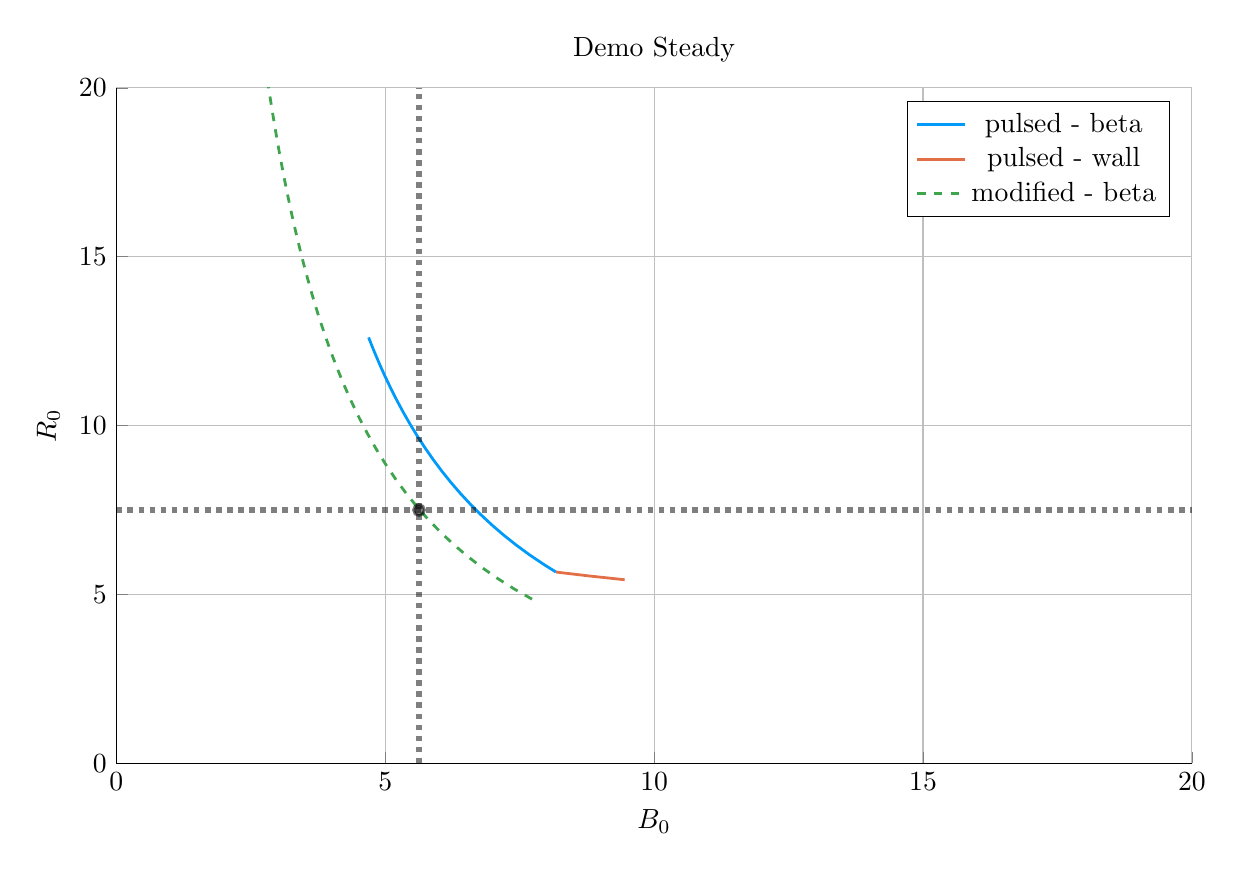
\begin{tikzpicture}[]
\begin{axis}[height = {101.6mm}, ylabel = {$R_0$}, title = {Demo Steady}, xmin = {0.0}, xmax = {20.0}, ymax = {20.0}, xlabel = {$B_0$}, {unbounded coords=jump, scaled x ticks = false, xticklabel style={rotate = 0}, xmajorgrids = true, xtick = {0.0,5.0,10.0,15.0,20.0}, xticklabels = {0,5,10,15,20}, xtick align = inside, axis lines* = left, scaled y ticks = false, yticklabel style={rotate = 0}, ymajorgrids = true, ytick = {0.0,5.0,10.0,15.0,20.0}, yticklabels = {0,5,10,15,20}, ytick align = inside, axis lines* = left,     xshift = 0.0mm,
    yshift = 0.0mm,
    axis background/.style={fill={rgb,1:red,1.00000000;green,1.00000000;blue,1.00000000}}
}, ymin = {0.0}, width = {152.4mm}]\addplot+ [color = {rgb,1:red,0.00000000;green,0.60560316;blue,0.97868012},
draw opacity=1.0,
line width=1,
solid,mark = none,
mark size = 2.0,
mark options = {
    color = {rgb,1:red,0.00000000;green,0.00000000;blue,0.00000000}, draw opacity = 1.0,
    fill = {rgb,1:red,0.00000000;green,0.60560316;blue,0.97868012}, fill opacity = 1.0,
    line width = 1,
    rotate = 0,
    solid
}]coordinates {
(8.173486873088942, 5.664794455960266)
(7.942780080136996, 5.894389477908349)
(7.682110747013332, 6.174587309854596)
(7.436076373351653, 6.4617259587740365)
(7.203701032854224, 6.7556817964635885)
(6.984087846006315, 7.056316762210614)
(6.776411507024863, 7.363478485110443)
(6.579911624110169, 7.677000456183209)
(6.393886772782909, 7.996702249919802)
(6.217689175869905, 8.322389794615686)
(6.050719935402341, 8.653855690575247)
(5.892424751644716, 8.990879574996331)
(5.742290072962272, 9.333228532083597)
(5.599839627496144, 9.680657546690735)
(5.464631293842628, 10.03290999955685)
(5.33625427328881, 10.389718201981736)
(5.214326530771975, 10.75080396758328)
(5.098492475718857, 11.115879218594692)
(4.98842085737482, 11.484646623994054)
(4.88380285223036, 11.85680026661456)
(4.784350323760147, 12.232026336259217)
(4.689794236961777, 12.610003845742904)
};
\addlegendentry{pulsed - beta}
\addplot+ [color = {rgb,1:red,0.88887350;green,0.43564919;blue,0.27812294},
draw opacity=1.0,
line width=1,
solid,mark = none,
mark size = 2.0,
mark options = {
    color = {rgb,1:red,0.00000000;green,0.00000000;blue,0.00000000}, draw opacity = 1.0,
    fill = {rgb,1:red,0.88887350;green,0.43564919;blue,0.27812294}, fill opacity = 1.0,
    line width = 1,
    rotate = 0,
    solid
}]coordinates {
(9.452194760190558, 5.436039445052516)
(8.82895875946862, 5.541751345019407)
(8.260410483462291, 5.64769543408014)
(8.173486873088942, 5.664794455960266)
};
\addlegendentry{pulsed - wall}
\addplot+ [color = {rgb,1:red,0.24222430;green,0.64327509;blue,0.30444865},
draw opacity=1.0,
line width=1,
dashed,mark = none,
mark size = 2.0,
mark options = {
    color = {rgb,1:red,0.00000000;green,0.00000000;blue,0.00000000}, draw opacity = 1.0,
    fill = {rgb,1:red,0.24222430;green,0.64327509;blue,0.30444865}, fill opacity = 1.0,
    line width = 1,
    rotate = 0,
    solid
}]coordinates {
(7.729015258613306, 4.861871150043874)
(7.398090906424027, 5.162615732748398)
(7.087604971989989, 5.475689582149146)
(6.796029845186129, 5.801261884855786)
(6.5219747916377235, 6.139486028413868)
(6.264171517105504, 6.490498735804173)
(6.021461495247516, 6.854419238072999)
(5.792784817023639, 7.231348485954994)
(5.57717035299729, 7.621368405021026)
(5.3737270519036775, 8.024541198865679)
(5.1816362256187425, 8.440908704652248)
(5.000144692923053, 8.870491805097014)
(4.828558673035444, 9.313289900712723)
(4.666238335465348, 9.769280445839089)
(4.512592925835539, 10.23841855166636)
(4.367076398389423, 10.720636659108127)
(4.229183495269078, 11.215844284001262)
(4.098446220614958, 11.723927836706606)
(3.974430664327246, 12.244750517759236)
(3.856734136133517, 12.778152290770123)
(3.744982575583214, 13.323949933321568)
(3.6388282078672565, 13.881937166125676)
(3.537947419047361, 14.45188486023713)
(3.4420388274654035, 15.033541321628862)
(3.3508215308612357, 15.626632651963563)
(3.2640335111230074, 16.230863183919308)
(3.18143018067718, 16.84591598897328)
(3.1027830563428513, 17.471453455103656)
(3.0278785480626333, 18.107117931452404)
(2.956516851312625, 18.752532436599008)
(2.888510933213844, 19.407301426734122)
(2.823685603439882, 20.071011619694055)
(2.761876661959762, 20.74323287052923)
(2.702930116488407, 21.423519094029906)
(2.646701463253573, 22.111409229427537)
(2.593055025340143, 22.806428242329144)
};
\addlegendentry{modified - beta}
\addplot+ [color = {rgb,1:red,0.00000000;green,0.00000000;blue,0.00000000},
draw opacity=0.5,
line width=2,
dotted,mark = none,
mark size = 2.0,
mark options = {
    color = {rgb,1:red,0.00000000;green,0.00000000;blue,0.00000000}, draw opacity = 0.5,
    fill = {rgb,1:red,0.00000000;green,0.00000000;blue,0.00000000}, fill opacity = 0.5,
    line width = 1,
    rotate = 0,
    solid
},forget plot]coordinates {
(0.0, 7.5)
(20.0, 7.5)
};
\addplot+ [color = {rgb,1:red,0.00000000;green,0.00000000;blue,0.00000000},
draw opacity=0.5,
line width=2,
dotted,mark = none,
mark size = 2.0,
mark options = {
    color = {rgb,1:red,0.00000000;green,0.00000000;blue,0.00000000}, draw opacity = 0.5,
    fill = {rgb,1:red,0.00000000;green,0.00000000;blue,0.00000000}, fill opacity = 0.5,
    line width = 1,
    rotate = 0,
    solid
},forget plot]coordinates {
(5.627, 0.0)
(5.627, 20.0)
};
\addplot+[draw=none, color = {rgb,1:red,0.00000000;green,0.00000000;blue,0.00000000},
draw opacity=0.5,
line width=0,
solid,mark = *,
mark size = 2.0,
mark options = {
    color = {rgb,1:red,0.00000000;green,0.00000000;blue,0.00000000}, draw opacity = 0.5,
    fill = {rgb,1:red,0.00000000;green,0.00000000;blue,0.00000000}, fill opacity = 0.5,
    line width = 1,
    rotate = 0,
    solid
},forget plot] coordinates {
(5.627, 7.5)
};
\end{axis}

\end{tikzpicture}

    \end{adjustbox}
        \caption{$R_0$ vs $B_0$}
    \end{subfigure}
    \hfill
    \begin{subfigure}[t]{0.45\textwidth}
        \centering
    \begin{adjustbox}{width=\textwidth}
      \Large
      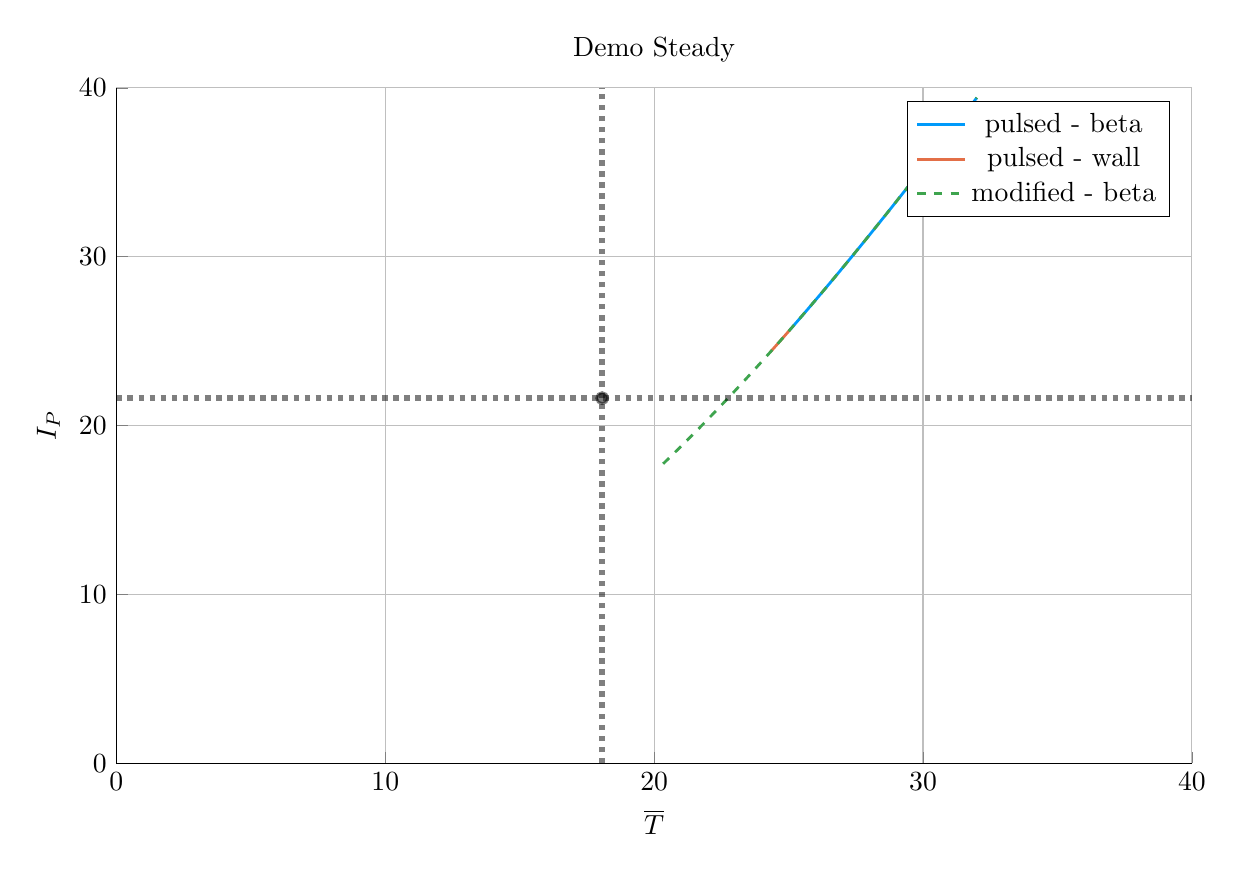
\begin{tikzpicture}[]
\begin{axis}[height = {101.6mm}, ylabel = {$I_P$}, title = {Demo Steady}, xmin = {0.0}, xmax = {40.0}, ymax = {40.0}, xlabel = {$\overline T$}, {unbounded coords=jump, scaled x ticks = false, xticklabel style={rotate = 0}, xmajorgrids = true, xtick = {0.0,10.0,20.0,30.0,40.0}, xticklabels = {0,10,20,30,40}, xtick align = inside, axis lines* = left, scaled y ticks = false, yticklabel style={rotate = 0}, ymajorgrids = true, ytick = {0.0,10.0,20.0,30.0,40.0}, yticklabels = {0,10,20,30,40}, ytick align = inside, axis lines* = left,     xshift = 0.0mm,
    yshift = 0.0mm,
    axis background/.style={fill={rgb,1:red,1.00000000;green,1.00000000;blue,1.00000000}}
}, ymin = {0.0}, width = {152.4mm}]\addplot+ [color = {rgb,1:red,0.00000000;green,0.60560316;blue,0.97868012},
draw opacity=1.0,
line width=1,
solid,mark = none,
mark size = 2.0,
mark options = {
    color = {rgb,1:red,0.00000000;green,0.00000000;blue,0.00000000}, draw opacity = 1.0,
    fill = {rgb,1:red,0.00000000;green,0.60560316;blue,0.97868012}, fill opacity = 1.0,
    line width = 1,
    rotate = 0,
    solid
}]coordinates {
(25.053735982163357, 25.677558860299992)
(25.333333333333332, 26.189593064380034)
(25.666666666666668, 26.80548085953921)
(26.0, 27.427148406840605)
(26.333333333333332, 28.054440831282633)
(26.666666666666668, 28.68719962041386)
(27.0, 29.325262818659787)
(27.333333333333332, 29.968465226287904)
(27.666666666666668, 30.6166386025962)
(28.0, 31.269611872884024)
(28.333333333333332, 31.92721133872904)
(28.666666666666668, 32.589260891064264)
(29.0, 33.25558222552837)
(29.333333333333332, 33.925995059549685)
(29.666666666666668, 34.60031735061725)
(30.0, 35.27836551518855)
(30.333333333333332, 35.95995464768734)
(30.666666666666668, 36.644898739049395)
(31.0, 37.333010894283476)
(31.333333333333332, 38.02410354852819)
(31.666666666666668, 38.717988681099214)
(32.0, 39.41447802704077)
};
\addlegendentry{pulsed - beta}
\addplot+ [color = {rgb,1:red,0.88887350;green,0.43564919;blue,0.27812294},
draw opacity=1.0,
line width=1,
solid,mark = none,
mark size = 2.0,
mark options = {
    color = {rgb,1:red,0.00000000;green,0.00000000;blue,0.00000000}, draw opacity = 1.0,
    fill = {rgb,1:red,0.88887350;green,0.43564919;blue,0.27812294}, fill opacity = 1.0,
    line width = 1,
    rotate = 0,
    solid
}]coordinates {
(24.333333333333332, 24.378107374495485)
(24.666666666666668, 24.975762903314084)
(25.0, 25.579637086786484)
(25.053735982163357, 25.677558860299992)
};
\addlegendentry{pulsed - wall}
\addplot+ [color = {rgb,1:red,0.24222430;green,0.64327509;blue,0.30444865},
draw opacity=1.0,
line width=1,
dashed,mark = none,
mark size = 2.0,
mark options = {
    color = {rgb,1:red,0.00000000;green,0.00000000;blue,0.00000000}, draw opacity = 1.0,
    fill = {rgb,1:red,0.24222430;green,0.64327509;blue,0.30444865}, fill opacity = 1.0,
    line width = 1,
    rotate = 0,
    solid
}]coordinates {
(20.333333333333332, 17.737142606162497)
(20.666666666666668, 18.250736761644205)
(21.0, 18.771889258341997)
(21.333333333333332, 19.300518519223587)
(21.666666666666668, 19.836537357082282)
(22.0, 20.37985305559639)
(22.333333333333332, 20.930367463801495)
(22.666666666666668, 21.487977099646507)
(23.0, 22.05257326267931)
(23.333333333333332, 22.62404215595106)
(23.666666666666668, 23.202265017123075)
(24.0, 23.787118258664318)
(24.333333333333332, 24.378473616949)
(24.666666666666668, 24.976198309995638)
(25.0, 25.58015520352756)
(25.333333333333332, 26.19020298497985)
(25.666666666666668, 26.806196345025047)
(26.0, 27.427986166140983)
(26.333333333333332, 28.055419717698932)
(26.666666666666668, 28.688340857006587)
(27.0, 29.3265902357016)
(27.333333333333332, 29.970005510854897)
(27.666666666666668, 30.61842156011136)
(28.0, 31.27167070016686)
(28.333333333333332, 31.92958290785876)
(28.666666666666668, 32.591986043126525)
(29.0, 33.25870607308836)
(29.333333333333332, 33.929567296470175)
(29.666666666666668, 34.604392567622554)
(30.0, 35.28300351936469)
(30.333333333333332, 35.96522078390488)
(30.666666666666668, 36.650864211102025)
(31.0, 37.3397530833557)
(31.333333333333332, 38.03170632643894)
(31.666666666666668, 38.726542715621264)
(32.0, 39.424081076468326)
};
\addlegendentry{modified - beta}
\addplot+ [color = {rgb,1:red,0.00000000;green,0.00000000;blue,0.00000000},
draw opacity=0.5,
line width=2,
dotted,mark = none,
mark size = 2.0,
mark options = {
    color = {rgb,1:red,0.00000000;green,0.00000000;blue,0.00000000}, draw opacity = 0.5,
    fill = {rgb,1:red,0.00000000;green,0.00000000;blue,0.00000000}, fill opacity = 0.5,
    line width = 1,
    rotate = 0,
    solid
},forget plot]coordinates {
(0.0, 21.627)
(40.0, 21.627)
};
\addplot+ [color = {rgb,1:red,0.00000000;green,0.00000000;blue,0.00000000},
draw opacity=0.5,
line width=2,
dotted,mark = none,
mark size = 2.0,
mark options = {
    color = {rgb,1:red,0.00000000;green,0.00000000;blue,0.00000000}, draw opacity = 0.5,
    fill = {rgb,1:red,0.00000000;green,0.00000000;blue,0.00000000}, fill opacity = 0.5,
    line width = 1,
    rotate = 0,
    solid
},forget plot]coordinates {
(18.067, 0.0)
(18.067, 40.0)
};
\addplot+[draw=none, color = {rgb,1:red,0.00000000;green,0.00000000;blue,0.00000000},
draw opacity=0.5,
line width=0,
solid,mark = *,
mark size = 2.0,
mark options = {
    color = {rgb,1:red,0.00000000;green,0.00000000;blue,0.00000000}, draw opacity = 0.5,
    fill = {rgb,1:red,0.00000000;green,0.00000000;blue,0.00000000}, fill opacity = 0.5,
    line width = 1,
    rotate = 0,
    solid
},forget plot] coordinates {
(18.067, 21.627)
};
\end{axis}

\end{tikzpicture}

    \end{adjustbox}
        \caption{$I_P$ vs $\overline T$}
    \end{subfigure}
    \hfill \hfill ~\\ ~\\ ~\\
    \caption{Demo Steady Model Comparison} ~\\
\end{figure*}

\begin{table}[h!]
\centering  
\caption{Demo Steady Variables}
\hfill
\begin{subtable}[t]{0.4\textwidth}
\centering  
\caption{Input Variables} ~\\
\begin{tabular}{ c|c } 

Input            & Value           \\
\hline
$H$              & 1.4             \\
$Q$              & 24.46           \\
$N_{G}$          & 1.2             \\
$\epsilon$       & 0.385           \\
$\kappa_{95}$    & 1.8             \\
$\delta_{95}$    & 0.333           \\
$\nu_{n}$        & 0.3972          \\
$\nu_{T}$        & 0.9187          \\
$l_{i}$          & 0.9             \\
$A$              & 2.856           \\
$Z_{eff}$        & 4.708           \\
$f_{D}$          & 0.7366          \\
$\tau_{FT}$      & 1.6e9           \\
$B_{CS}$         & 12.85           \\

\end{tabular}
\end{subtable}
\hfill
\begin{subtable}[t]{0.5\textwidth}
\centering  
\caption{Output Variables} ~\\
\begin{tabular}{ c|c|c } 

Output           & Original         & Fussy.jl        \\  
\hline
$R_{0}$          & 7.5              & 8.154           \\
$B_{0}$          & 5.627            & 6.307           \\
$I_{P}$          & 21.63            & 30.93           \\
$\overline n$    & 0.8746           & 1.048           \\
$\overline T$    & 18.07            & 27.83           \\
$\beta_{N}$       & 0.038            & 0.038           \\
$q_{95}$         & 4.405            & 3.761           \\
$P_{W}$          & 1.911            & 4.151           \\
$f_{BS}$         & 0.611            & 0.4241          \\
$f_{CD}$         & 0.389            & 0.5759          \\
$f_{IN}$         & -              & -             \\
$\volume$         & 2217           & 2879          \\
$P_{F}$          & 3255           & 8971          \\
$\eta_{CD}$      & 0.4152           & -          \\

\end{tabular}
\end{subtable}
\hfill
\hfill
\end{table}

\newpage 

\subsubsection{DEMO Pulsed -- A Pulsed ITER Successor}

\begin{figure*}[h!]
    \centering
    \hfill 
    \begin{subfigure}[t]{0.45\textwidth}
        \centering
    \begin{adjustbox}{width=\textwidth}
      \Large
      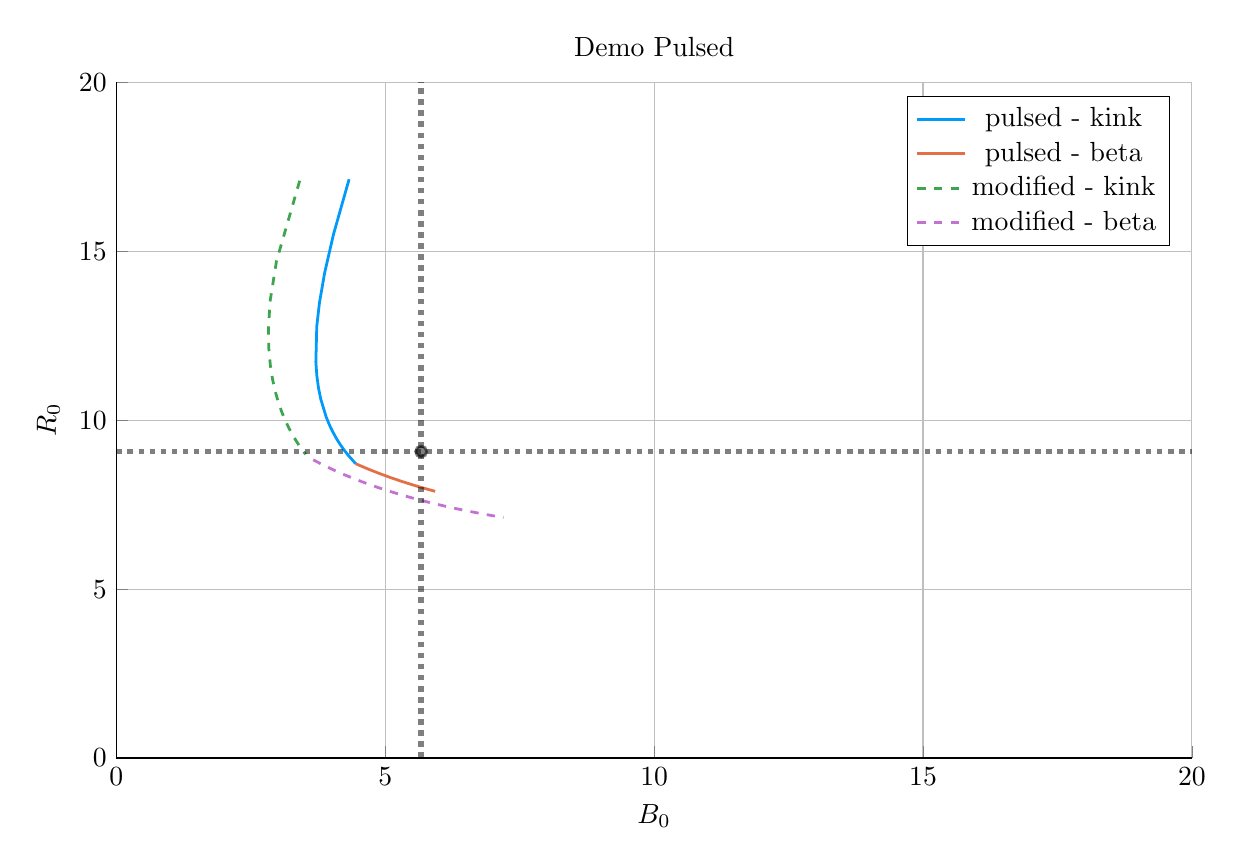
\begin{tikzpicture}[]
\begin{axis}[height = {101.6mm}, ylabel = {$R_0$}, title = {Demo Pulsed}, xmin = {0.0}, xmax = {20.0}, ymax = {20.0}, xlabel = {$B_0$}, {unbounded coords=jump, scaled x ticks = false, xticklabel style={rotate = 0}, xmajorgrids = true, xtick = {0.0,5.0,10.0,15.0,20.0}, xticklabels = {0,5,10,15,20}, xtick align = inside, axis lines* = left, scaled y ticks = false, yticklabel style={rotate = 0}, ymajorgrids = true, ytick = {0.0,5.0,10.0,15.0,20.0}, yticklabels = {0,5,10,15,20}, ytick align = inside, axis lines* = left,     xshift = 0.0mm,
    yshift = 0.0mm,
    axis background/.style={fill={rgb,1:red,1.00000000;green,1.00000000;blue,1.00000000}}
}, ymin = {0.0}, width = {152.4mm}]\addplot+ [color = {rgb,1:red,0.00000000;green,0.60560316;blue,0.97868012},
draw opacity=1.0,
line width=1,
solid,mark = none,
mark size = 2.0,
mark options = {
    color = {rgb,1:red,0.00000000;green,0.00000000;blue,0.00000000}, draw opacity = 1.0,
    fill = {rgb,1:red,0.00000000;green,0.60560316;blue,0.97868012}, fill opacity = 1.0,
    line width = 1,
    rotate = 0,
    solid
}]coordinates {
(4.327031075670194, 17.134796748649162)
(4.038214026054326, 15.511755022601415)
(3.8713719163129245, 14.355562963913712)
(3.7758613845615545, 13.476675762289453)
(3.7257856761317214, 12.778294295391971)
(3.7090473695925437, 11.723065749829066)
(3.727711597554826, 11.30970201784727)
(3.7586131667481433, 10.94971275897184)
(3.799052518631718, 10.632190690377048)
(3.901290136389271, 10.09455415135144)
(3.960577465316514, 9.863813619410237)
(4.0241209645210345, 9.653307397969705)
(4.0912717805663785, 9.460162902699798)
(4.161514602943343, 9.28206292757184)
(4.2344343960723005, 9.117114543572253)
(4.309692554546368, 8.963753917462126)
(4.450417240491067, 8.712493965092264)
};
\addlegendentry{pulsed - kink}
\addplot+ [color = {rgb,1:red,0.88887350;green,0.43564919;blue,0.27812294},
draw opacity=1.0,
line width=1,
solid,mark = none,
mark size = 2.0,
mark options = {
    color = {rgb,1:red,0.00000000;green,0.00000000;blue,0.00000000}, draw opacity = 1.0,
    fill = {rgb,1:red,0.88887350;green,0.43564919;blue,0.27812294}, fill opacity = 1.0,
    line width = 1,
    rotate = 0,
    solid
}]coordinates {
(4.450417240491067, 8.712493965092264)
(4.490148631384312, 8.684308742646298)
(4.692490181445514, 8.547262773806349)
(4.8960344619053355, 8.41947837460442)
(5.100651132702229, 8.30014929484307)
(5.306202822090688, 8.188581738801314)
(5.512545696627038, 8.084175191078112)
(5.719530043226767, 7.986407002697611)
(5.927000883375481, 7.894819882619234)
};
\addlegendentry{pulsed - beta}
\addplot+ [color = {rgb,1:red,0.24222430;green,0.64327509;blue,0.30444865},
draw opacity=1.0,
line width=1,
dashed,mark = none,
mark size = 2.0,
mark options = {
    color = {rgb,1:red,0.00000000;green,0.00000000;blue,0.00000000}, draw opacity = 1.0,
    fill = {rgb,1:red,0.24222430;green,0.64327509;blue,0.30444865}, fill opacity = 1.0,
    line width = 1,
    rotate = 0,
    solid
}]coordinates {
(3.4087424183072135, 17.090884129081292)
(2.977074181068944, 14.713048632784332)
(2.8592500074202523, 13.541171522519205)
(2.827199220063259, 12.740024138753894)
(2.8339789008667826, 12.12574468151967)
(2.862412302880871, 11.626187613249266)
(2.9044598258085443, 11.205091848948229)
(2.95577893007882, 10.841432203317366)
(3.0137895352525907, 10.521822649209419)
(3.076849710218805, 10.23716073884787)
(3.1438583711612704, 9.980947801083442)
(3.214045733980633, 9.748367275345563)
(3.2868548955983727, 9.535742205343247)
(3.361871149981842, 9.340197658526863)
(3.4387778750377818, 9.15944098345979)
(3.5173279629378453, 8.991613349767409)
};
\addlegendentry{modified - kink}
\addplot+ [color = {rgb,1:red,0.76444018;green,0.44411178;blue,0.82429754},
draw opacity=1.0,
line width=1,
dashed,mark = none,
mark size = 2.0,
mark options = {
    color = {rgb,1:red,0.00000000;green,0.00000000;blue,0.00000000}, draw opacity = 1.0,
    fill = {rgb,1:red,0.76444018;green,0.44411178;blue,0.82429754}, fill opacity = 1.0,
    line width = 1,
    rotate = 0,
    solid
}]coordinates {
(3.6607028750648505, 8.825949645171955)
(3.8574448036470477, 8.664618827122876)
(4.056375867871351, 8.51434867582932)
(4.257366397480293, 8.374075613831488)
(4.460279103534801, 8.242896218794312)
(4.664969389370631, 8.12003771613466)
(4.871285596007394, 8.004834914067093)
(5.07906923307514, 7.896711937521184)
(5.288155233306219, 7.795167587687744)
(5.498372259673351, 7.699763475973523)
(5.709543087166185, 7.610114306522102)
(5.921485076209294, 7.525879840414137)
(6.134010749367255, 7.446758190646709)
(6.346928478632384, 7.372480180910637)
(6.560043285872518, 7.302804563889649)
(6.773157754368795, 7.237513941672651)
(6.986073044284746, 7.176411266758267)
(7.198590001107076, 7.119316828230052)
};
\addlegendentry{modified - beta}
\addplot+ [color = {rgb,1:red,0.00000000;green,0.00000000;blue,0.00000000},
draw opacity=0.5,
line width=2,
dotted,mark = none,
mark size = 2.0,
mark options = {
    color = {rgb,1:red,0.00000000;green,0.00000000;blue,0.00000000}, draw opacity = 0.5,
    fill = {rgb,1:red,0.00000000;green,0.00000000;blue,0.00000000}, fill opacity = 0.5,
    line width = 1,
    rotate = 0,
    solid
},forget plot]coordinates {
(0.0, 9.072)
(20.0, 9.072)
};
\addplot+ [color = {rgb,1:red,0.00000000;green,0.00000000;blue,0.00000000},
draw opacity=0.5,
line width=2,
dotted,mark = none,
mark size = 2.0,
mark options = {
    color = {rgb,1:red,0.00000000;green,0.00000000;blue,0.00000000}, draw opacity = 0.5,
    fill = {rgb,1:red,0.00000000;green,0.00000000;blue,0.00000000}, fill opacity = 0.5,
    line width = 1,
    rotate = 0,
    solid
},forget plot]coordinates {
(5.667, 0.0)
(5.667, 20.0)
};
\addplot+[draw=none, color = {rgb,1:red,0.00000000;green,0.00000000;blue,0.00000000},
draw opacity=0.5,
line width=0,
solid,mark = *,
mark size = 2.0,
mark options = {
    color = {rgb,1:red,0.00000000;green,0.00000000;blue,0.00000000}, draw opacity = 0.5,
    fill = {rgb,1:red,0.00000000;green,0.00000000;blue,0.00000000}, fill opacity = 0.5,
    line width = 1,
    rotate = 0,
    solid
},forget plot] coordinates {
(5.667, 9.072)
};
\end{axis}

\end{tikzpicture}

    \end{adjustbox}
        \caption{$R_0$ vs $B_0$}
    \end{subfigure}
    \hfill
    \begin{subfigure}[t]{0.45\textwidth}
        \centering
    \begin{adjustbox}{width=\textwidth}
      \Large
      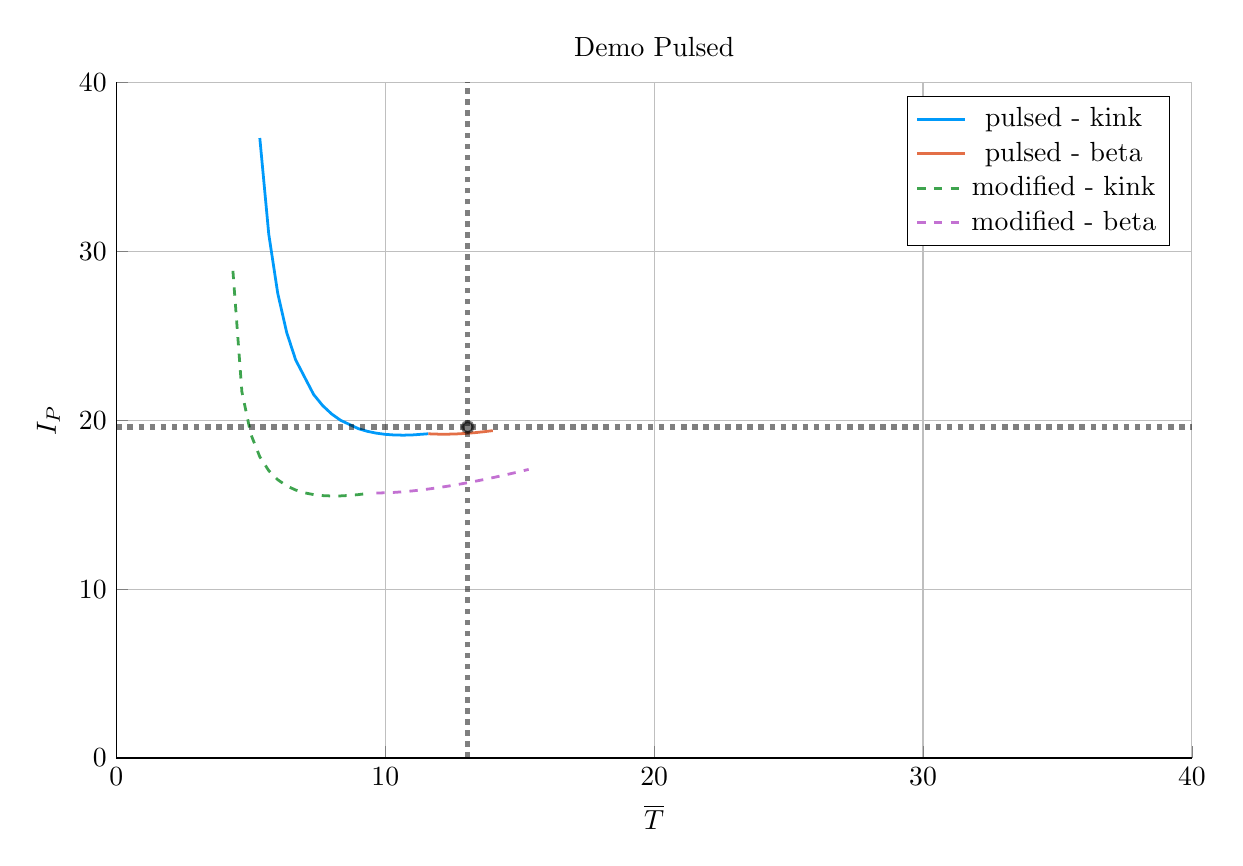
\begin{tikzpicture}[]
\begin{axis}[height = {101.6mm}, ylabel = {$I_P$}, title = {Demo Pulsed}, xmin = {0.0}, xmax = {40.0}, ymax = {40.0}, xlabel = {$\overline T$}, {unbounded coords=jump, scaled x ticks = false, xticklabel style={rotate = 0}, xmajorgrids = true, xtick = {0.0,10.0,20.0,30.0,40.0}, xticklabels = {0,10,20,30,40}, xtick align = inside, axis lines* = left, scaled y ticks = false, yticklabel style={rotate = 0}, ymajorgrids = true, ytick = {0.0,10.0,20.0,30.0,40.0}, yticklabels = {0,10,20,30,40}, ytick align = inside, axis lines* = left,     xshift = 0.0mm,
    yshift = 0.0mm,
    axis background/.style={fill={rgb,1:red,1.00000000;green,1.00000000;blue,1.00000000}}
}, ymin = {0.0}, width = {152.4mm}]\addplot+ [color = {rgb,1:red,0.00000000;green,0.60560316;blue,0.97868012},
draw opacity=1.0,
line width=1,
solid,mark = none,
mark size = 2.0,
mark options = {
    color = {rgb,1:red,0.00000000;green,0.00000000;blue,0.00000000}, draw opacity = 1.0,
    fill = {rgb,1:red,0.00000000;green,0.60560316;blue,0.97868012}, fill opacity = 1.0,
    line width = 1,
    rotate = 0,
    solid
}]coordinates {
(5.333333333333333, 36.71051032912112)
(5.666666666666667, 31.014995367356207)
(6.0, 27.51734786322149)
(6.333333333333333, 25.19534286389616)
(6.666666666666667, 23.57285610926683)
(7.333333333333333, 21.52905816503197)
(7.666666666666667, 20.874444053021588)
(8.0, 20.377542510464334)
(8.333333333333334, 19.99951688957442)
(9.0, 19.499202175706746)
(9.333333333333334, 19.343044014643887)
(9.666666666666666, 19.233955791269285)
(10.0, 19.16365729524907)
(10.333333333333334, 19.125701869840853)
(10.666666666666666, 19.11499858904485)
(11.0, 19.127475979338943)
(11.600962879632572, 19.198383823705257)
};
\addlegendentry{pulsed - kink}
\addplot+ [color = {rgb,1:red,0.88887350;green,0.43564919;blue,0.27812294},
draw opacity=1.0,
line width=1,
solid,mark = none,
mark size = 2.0,
mark options = {
    color = {rgb,1:red,0.00000000;green,0.00000000;blue,0.00000000}, draw opacity = 1.0,
    fill = {rgb,1:red,0.88887350;green,0.43564919;blue,0.27812294}, fill opacity = 1.0,
    line width = 1,
    rotate = 0,
    solid
}]coordinates {
(11.600962879632572, 19.198383823705257)
(11.666666666666666, 19.192414153878335)
(12.0, 19.174087186739918)
(12.333333333333334, 19.17397121853779)
(12.666666666666666, 19.189978018951553)
(13.0, 19.220357277326283)
(13.333333333333334, 19.263633100211838)
(13.666666666666666, 19.31855421750887)
(14.0, 19.384054548489104)
};
\addlegendentry{pulsed - beta}
\addplot+ [color = {rgb,1:red,0.24222430;green,0.64327509;blue,0.30444865},
draw opacity=1.0,
line width=1,
dashed,mark = none,
mark size = 2.0,
mark options = {
    color = {rgb,1:red,0.00000000;green,0.00000000;blue,0.00000000}, draw opacity = 1.0,
    fill = {rgb,1:red,0.24222430;green,0.64327509;blue,0.30444865}, fill opacity = 1.0,
    line width = 1,
    rotate = 0,
    solid
}]coordinates {
(4.333333333333333, 28.845639077165217)
(4.666666666666667, 21.687713986294685)
(5.0, 19.170340224057398)
(5.333333333333333, 17.83397336320386)
(5.666666666666667, 17.01478565989059)
(6.0, 16.477486603636205)
(6.333333333333333, 16.113958654578386)
(6.666666666666667, 15.866460603971907)
(7.0, 15.700928946757587)
(7.333333333333333, 15.59578560596909)
(7.666666666666667, 15.536607983152381)
(8.0, 15.513342675582972)
(8.333333333333334, 15.518740955012225)
(8.666666666666666, 15.547428978968492)
(9.0, 15.595329068459918)
(9.333333333333334, 15.659285368310089)
};
\addlegendentry{modified - kink}
\addplot+ [color = {rgb,1:red,0.76444018;green,0.44411178;blue,0.82429754},
draw opacity=1.0,
line width=1,
dashed,mark = none,
mark size = 2.0,
mark options = {
    color = {rgb,1:red,0.00000000;green,0.00000000;blue,0.00000000}, draw opacity = 1.0,
    fill = {rgb,1:red,0.76444018;green,0.44411178;blue,0.82429754}, fill opacity = 1.0,
    line width = 1,
    rotate = 0,
    solid
}]coordinates {
(9.666666666666666, 15.691192911261952)
(10.0, 15.70165788278533)
(10.333333333333334, 15.726578234093749)
(10.666666666666666, 15.764127054896537)
(11.0, 15.812802650736373)
(11.333333333333334, 15.871360766004056)
(11.666666666666666, 15.938763317563621)
(12.0, 16.014139065408)
(12.333333333333334, 16.09675304572932)
(12.666666666666666, 16.185982524147033)
(13.0, 16.281297862810217)
(13.333333333333334, 16.382247130746602)
(13.666666666666666, 16.488443597982137)
(14.0, 16.5995554722192)
(14.333333333333334, 16.715297396529092)
(14.666666666666666, 16.83542334285969)
(15.0, 16.959720624053933)
(15.333333333333334, 17.088004807739882)
};
\addlegendentry{modified - beta}
\addplot+ [color = {rgb,1:red,0.00000000;green,0.00000000;blue,0.00000000},
draw opacity=0.5,
line width=2,
dotted,mark = none,
mark size = 2.0,
mark options = {
    color = {rgb,1:red,0.00000000;green,0.00000000;blue,0.00000000}, draw opacity = 0.5,
    fill = {rgb,1:red,0.00000000;green,0.00000000;blue,0.00000000}, fill opacity = 0.5,
    line width = 1,
    rotate = 0,
    solid
},forget plot]coordinates {
(0.0, 19.6)
(40.0, 19.6)
};
\addplot+ [color = {rgb,1:red,0.00000000;green,0.00000000;blue,0.00000000},
draw opacity=0.5,
line width=2,
dotted,mark = none,
mark size = 2.0,
mark options = {
    color = {rgb,1:red,0.00000000;green,0.00000000;blue,0.00000000}, draw opacity = 0.5,
    fill = {rgb,1:red,0.00000000;green,0.00000000;blue,0.00000000}, fill opacity = 0.5,
    line width = 1,
    rotate = 0,
    solid
},forget plot]coordinates {
(13.065, 0.0)
(13.065, 40.0)
};
\addplot+[draw=none, color = {rgb,1:red,0.00000000;green,0.00000000;blue,0.00000000},
draw opacity=0.5,
line width=0,
solid,mark = *,
mark size = 2.0,
mark options = {
    color = {rgb,1:red,0.00000000;green,0.00000000;blue,0.00000000}, draw opacity = 0.5,
    fill = {rgb,1:red,0.00000000;green,0.00000000;blue,0.00000000}, fill opacity = 0.5,
    line width = 1,
    rotate = 0,
    solid
},forget plot] coordinates {
(13.065, 19.6)
};
\end{axis}

\end{tikzpicture}

    \end{adjustbox}
        \caption{$I_P$ vs $\overline T$}
    \end{subfigure}
    \hfill \hfill ~\\ ~\\ ~\\
    \caption{Demo Pulsed Model Comparison} ~\\
\end{figure*}

\begin{table}[h!]
\centering  
\caption{Demo Pulsed Variables}
\hfill
\begin{subtable}[t]{0.4\textwidth}
\centering  
\caption{Input Variables} ~\\
\begin{tabular}{ c|c } 

Input            & Value           \\
\hline
$H$              & 1.1             \\
$Q$              & 39.86           \\
$N_{G}$          & 1.2             \\
$\epsilon$       & 0.3226          \\
$\kappa_{95}$    & 1.59            \\
$\delta_{95}$    & 0.333           \\
$\nu_{n}$        & 0.27            \\
$\nu_{T}$        & 1.094           \\
$l_{i}$          & 1.155           \\
$A$              & 2.735           \\
$Z_{eff}$        & 2.584           \\
$f_{D}$          & 0.7753          \\
$\tau_{FT}$      & 7273          \\
$B_{CS}$         & 12.77           \\

\end{tabular}
\end{subtable}
\hfill
\begin{subtable}[t]{0.5\textwidth}
\centering  
\caption{Output Variables} ~\\
\begin{tabular}{ c|c|c } 

Output           & Original         & Fussy.jl        \\
\hline
$R_{0}$          & 9.072            & 8.1             \\
$B_{0}$          & 5.667            & 5.48            \\
$I_{P}$          & 19.6             & 19.26           \\
$\overline n$    & 0.7983           & 0.9795          \\
$\overline T$    & 13.06            & 13.28           \\
$\beta_{N}$       & 0.0259           & 0.0259          \\
$q_{95}$         & 3.247            & 2.853           \\
$P_{W}$          & 1.05             & 1.466           \\
$f_{BS}$         & 0.348            & 0.1637          \\
$f_{CD}$         & 0.096            & 0.1062          \\
$f_{IN}$         & 0.557            & 0.7302          \\
$\volume$         & 2502           & 1751          \\
$P_{F}$          & 2037           & 2376          \\
$\eta_{CD}$      & 0.2721           & -     

\end{tabular}
\end{subtable}
\hfill
\hfill
\end{table}

\section{Developing Prototype Reactors}

\begin{figure}[h!]
\centering
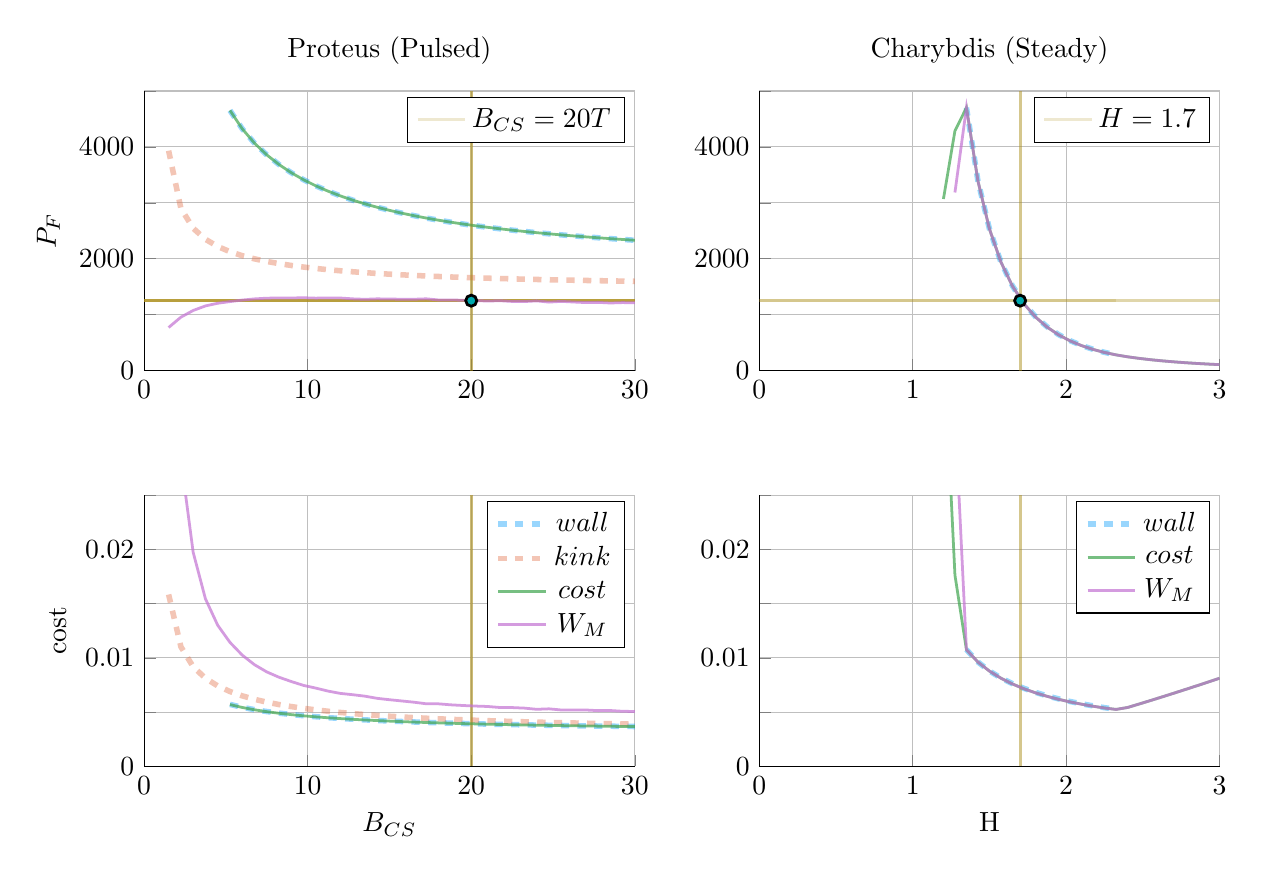
\begin{tikzpicture}[]
\begin{axis}[height = {51.32916666666667mm}, ylabel = {$P_F$}, title = {Proteus (Pulsed)}, xmin = {0}, xmax = {30.0}, ymax = {5000.0}, xlabel = {}, {unbounded coords=jump, scaled x ticks = false, xticklabel style={rotate = 0}, xmajorgrids = true, xtick = {0.0,10.0,20.0,30.0}, xticklabels = {0,10,20,30}, xtick align = inside, axis lines* = left, scaled y ticks = false, yticklabel style={rotate = 0}, ymajorgrids = true, ytick = {0,1000,2000,3000,4000,5000}, yticklabels = {0,,2000,,4000,}, ytick align = inside, axis lines* = left,     xshift = 0.0mm,
    yshift = 50.27mm,
    axis background/.style={fill={rgb,1:red,1.00000000;green,1.00000000;blue,1.00000000}}
}, ymin = {2.220446049250313e-16}, width = {78.14027777777778mm}]\addplot+ [color = {rgb,1:red,0.67554396;green,0.55566233;blue,0.09423434},
draw opacity=0.2,
line width=1,
solid,mark = none,
mark size = 2.0,
mark options = {
    color = {rgb,1:red,0.00000000;green,0.00000000;blue,0.00000000}, draw opacity = 1.0,
    fill = {rgb,1:red,0.67554396;green,0.55566233;blue,0.09423434}, fill opacity = 1.0,
    line width = 1,
    rotate = 0,
    solid
}]coordinates {
(20.0, 2.220446049250313e-16)
(20.0, 5000.0)
};
\addlegendentry{$B_{CS} = 20 T$}
\addplot+ [color = {rgb,1:red,0.67554396;green,0.55566233;blue,0.09423434},
draw opacity=0.2,
line width=1,
solid,mark = none,
mark size = 2.0,
mark options = {
    color = {rgb,1:red,0.00000000;green,0.00000000;blue,0.00000000}, draw opacity = 1.0,
    fill = {rgb,1:red,0.67554396;green,0.55566233;blue,0.09423434}, fill opacity = 1.0,
    line width = 1,
    rotate = 0,
    solid
},forget plot]coordinates {
(0.0, 1250.0)
(30.0, 1250.0)
};
\addplot+[draw=none, color = {rgb,1:red,0.00000048;green,0.66575898;blue,0.68099695},
draw opacity=1.0,
line width=0,
solid,mark = *,
mark size = 2.0,
mark options = {
    color = {rgb,1:red,0.00000000;green,0.00000000;blue,0.00000000}, draw opacity = 1.0,
    fill = {rgb,1:red,0.00000048;green,0.66575898;blue,0.68099695}, fill opacity = 1.0,
    line width = 1,
    rotate = 0,
    solid
},forget plot] coordinates {
(20, 1250)
};
\addplot+ [color = {rgb,1:red,0.67554396;green,0.55566233;blue,0.09423434},
draw opacity=0.2,
line width=1,
solid,mark = none,
mark size = 2.0,
mark options = {
    color = {rgb,1:red,0.00000000;green,0.00000000;blue,0.00000000}, draw opacity = 1.0,
    fill = {rgb,1:red,0.67554396;green,0.55566233;blue,0.09423434}, fill opacity = 1.0,
    line width = 1,
    rotate = 0,
    solid
},forget plot]coordinates {
(0.0, 1250.0)
(30.0, 1250.0)
};
\addplot+ [color = {rgb,1:red,0.00000000;green,0.60560316;blue,0.97868012},
draw opacity=0.4,
line width=2,
dashed,mark = none,
mark size = 2.0,
mark options = {
    color = {rgb,1:red,0.00000000;green,0.00000000;blue,0.00000000}, draw opacity = 1.0,
    fill = {rgb,1:red,0.00000000;green,0.60560316;blue,0.97868012}, fill opacity = 1.0,
    line width = 1,
    rotate = 0,
    solid
},forget plot]coordinates {
(5.25, 4651.734735476011)
(6.0, 4323.6250098364)
(6.75, 4065.99692078527)
(7.5, 3857.273578687972)
(8.25, 3684.1342593418663)
(9.0, 3537.844669896544)
(9.75, 3412.404653539425)
(10.5, 3303.536032694244)
(11.25, 3208.094051273514)
(12.0, 3123.707522754923)
(12.75, 3048.5495054628623)
(13.5, 2981.185980181023)
(14.25, 2920.472987010462)
(15.0, 2865.484885250518)
(15.75, 2815.463186166668)
(16.5, 2769.7793320244814)
(17.25, 2727.9071420752607)
(18.0, 2689.4020933235493)
(18.75, 2653.885520176901)
(19.5, 2621.0324111911764)
(20.25, 2590.561874678777)
(21.0, 2562.2296107375955)
(21.75, 2535.8219099446264)
(22.5, 2511.150826555893)
(23.25, 2488.050264495335)
(24.0, 2466.372779394113)
(24.75, 2445.986947213969)
(25.5, 2426.775184780072)
(26.25, 2408.6319334297787)
(27.0, 2391.4621364565396)
(27.75, 2375.1799557182867)
(28.5, 2359.707684182671)
(29.25, 2344.974819785335)
(30.0, 2330.917272823136)
};
\addplot+ [color = {rgb,1:red,0.67554396;green,0.55566233;blue,0.09423434},
draw opacity=0.2,
line width=1,
solid,mark = none,
mark size = 2.0,
mark options = {
    color = {rgb,1:red,0.00000000;green,0.00000000;blue,0.00000000}, draw opacity = 1.0,
    fill = {rgb,1:red,0.67554396;green,0.55566233;blue,0.09423434}, fill opacity = 1.0,
    line width = 1,
    rotate = 0,
    solid
},forget plot]coordinates {
(20.0, 2.220446049250313e-16)
(20.0, 5000.0)
};
\addplot+ [color = {rgb,1:red,0.67554396;green,0.55566233;blue,0.09423434},
draw opacity=0.2,
line width=1,
solid,mark = none,
mark size = 2.0,
mark options = {
    color = {rgb,1:red,0.00000000;green,0.00000000;blue,0.00000000}, draw opacity = 1.0,
    fill = {rgb,1:red,0.67554396;green,0.55566233;blue,0.09423434}, fill opacity = 1.0,
    line width = 1,
    rotate = 0,
    solid
},forget plot]coordinates {
(0.0, 1250.0)
(30.0, 1250.0)
};
\addplot+ [color = {rgb,1:red,0.67554396;green,0.55566233;blue,0.09423434},
draw opacity=0.2,
line width=1,
solid,mark = none,
mark size = 2.0,
mark options = {
    color = {rgb,1:red,0.00000000;green,0.00000000;blue,0.00000000}, draw opacity = 1.0,
    fill = {rgb,1:red,0.67554396;green,0.55566233;blue,0.09423434}, fill opacity = 1.0,
    line width = 1,
    rotate = 0,
    solid
},forget plot]coordinates {
(0.0, 1250.0)
(30.0, 1250.0)
};
\addplot+ [color = {rgb,1:red,0.88887350;green,0.43564919;blue,0.27812294},
draw opacity=0.4,
line width=2,
dashed,mark = none,
mark size = 2.0,
mark options = {
    color = {rgb,1:red,0.00000000;green,0.00000000;blue,0.00000000}, draw opacity = 1.0,
    fill = {rgb,1:red,0.88887350;green,0.43564919;blue,0.27812294}, fill opacity = 1.0,
    line width = 1,
    rotate = 0,
    solid
},forget plot]coordinates {
(1.5, 3931.6170696070676)
(2.25, 2900.7235747979908)
(3.0, 2544.8446560898715)
(3.75, 2348.228116500571)
(4.5, 2219.0134794713767)
(5.25, 2125.815532966674)
(6.0, 2054.566085735622)
(6.75, 1997.8824990557177)
(7.5, 1951.4633680592258)
(8.25, 1912.6074536455505)
(9.0, 1879.5196356674505)
(9.75, 1850.953068441656)
(10.5, 1826.0101459658863)
(11.25, 1804.02551415983)
(12.0, 1784.493638745381)
(12.75, 1767.0222758941622)
(13.5, 1751.3015387280175)
(14.25, 1737.0827328069474)
(15.0, 1724.1634044428295)
(15.75, 1712.376890482151)
(16.5, 1701.5841921715175)
(17.25, 1691.6685698179294)
(18.0, 1682.530881991843)
(18.75, 1674.0861755860074)
(19.5, 1666.2615100001372)
(20.25, 1658.9932835127363)
(21.0, 1652.2262595201232)
(21.75, 1645.91179207308)
(22.5, 1640.0070406407558)
(23.25, 1634.4738680952948)
(24.0, 1629.2785569006053)
(24.75, 1624.3908184475338)
(25.5, 1619.7835209277835)
(26.25, 1615.432247074283)
(27.0, 1611.314956936522)
(27.75, 1607.4117026157203)
(28.5, 1603.7043856927105)
(29.25, 1600.1765499289672)
(30.0, 1596.813203261599)
};
\addplot+ [color = {rgb,1:red,0.67554396;green,0.55566233;blue,0.09423434},
draw opacity=0.2,
line width=1,
solid,mark = none,
mark size = 2.0,
mark options = {
    color = {rgb,1:red,0.00000000;green,0.00000000;blue,0.00000000}, draw opacity = 1.0,
    fill = {rgb,1:red,0.67554396;green,0.55566233;blue,0.09423434}, fill opacity = 1.0,
    line width = 1,
    rotate = 0,
    solid
},forget plot]coordinates {
(20.0, 2.220446049250313e-16)
(20.0, 5000.0)
};
\addplot+ [color = {rgb,1:red,0.67554396;green,0.55566233;blue,0.09423434},
draw opacity=0.2,
line width=1,
solid,mark = none,
mark size = 2.0,
mark options = {
    color = {rgb,1:red,0.00000000;green,0.00000000;blue,0.00000000}, draw opacity = 1.0,
    fill = {rgb,1:red,0.67554396;green,0.55566233;blue,0.09423434}, fill opacity = 1.0,
    line width = 1,
    rotate = 0,
    solid
},forget plot]coordinates {
(0.0, 1250.0)
(30.0, 1250.0)
};
\addplot+ [color = {rgb,1:red,0.67554396;green,0.55566233;blue,0.09423434},
draw opacity=0.2,
line width=1,
solid,mark = none,
mark size = 2.0,
mark options = {
    color = {rgb,1:red,0.00000000;green,0.00000000;blue,0.00000000}, draw opacity = 1.0,
    fill = {rgb,1:red,0.67554396;green,0.55566233;blue,0.09423434}, fill opacity = 1.0,
    line width = 1,
    rotate = 0,
    solid
},forget plot]coordinates {
(0.0, 1250.0)
(30.0, 1250.0)
};
\addplot+ [color = {rgb,1:red,0.24222430;green,0.64327509;blue,0.30444865},
draw opacity=0.7,
line width=1,
solid,mark = none,
mark size = 2.0,
mark options = {
    color = {rgb,1:red,0.00000000;green,0.00000000;blue,0.00000000}, draw opacity = 1.0,
    fill = {rgb,1:red,0.24222430;green,0.64327509;blue,0.30444865}, fill opacity = 1.0,
    line width = 1,
    rotate = 0,
    solid
},forget plot]coordinates {
(5.25, 4651.856974626446)
(6.0, 4323.626574700689)
(6.75, 4065.9133365013354)
(7.5, 3857.1264771824617)
(8.25, 3683.9377449687768)
(9.0, 3537.608432111376)
(9.75, 3412.1356303067523)
(10.5, 3303.239361854739)
(11.25, 3207.7736468791713)
(12.0, 3123.3664382128795)
(12.75, 3048.1901722862794)
(13.5, 2980.810371417949)
(14.25, 2920.082728006143)
(15.0, 2865.081335141082)
(15.75, 2815.0474968726217)
(16.5, 2769.352491750233)
(17.25, 2727.4700069605415)
(18.0, 2688.955412764386)
(18.75, 2653.4299583736)
(19.5, 2620.5685580410595)
(20.25, 2590.0902617025704)
(21.0, 2561.7507209540713)
(21.75, 2535.3361812985195)
(22.5, 2510.65866319561)
(23.25, 2487.5520396570964)
(24.0, 2465.868837737164)
(24.75, 2445.477613655657)
(25.5, 2426.2607621440256)
(26.25, 2408.1127073411044)
(27.0, 2390.9383771738235)
(27.75, 2374.651919394813)
(28.5, 2359.1756148307045)
(29.25, 2344.438950143004)
(30.0, 2330.377825995788)
};
\addplot+ [color = {rgb,1:red,0.67554396;green,0.55566233;blue,0.09423434},
draw opacity=0.2,
line width=1,
solid,mark = none,
mark size = 2.0,
mark options = {
    color = {rgb,1:red,0.00000000;green,0.00000000;blue,0.00000000}, draw opacity = 1.0,
    fill = {rgb,1:red,0.67554396;green,0.55566233;blue,0.09423434}, fill opacity = 1.0,
    line width = 1,
    rotate = 0,
    solid
},forget plot]coordinates {
(20.0, 2.220446049250313e-16)
(20.0, 5000.0)
};
\addplot+ [color = {rgb,1:red,0.67554396;green,0.55566233;blue,0.09423434},
draw opacity=0.2,
line width=1,
solid,mark = none,
mark size = 2.0,
mark options = {
    color = {rgb,1:red,0.00000000;green,0.00000000;blue,0.00000000}, draw opacity = 1.0,
    fill = {rgb,1:red,0.67554396;green,0.55566233;blue,0.09423434}, fill opacity = 1.0,
    line width = 1,
    rotate = 0,
    solid
},forget plot]coordinates {
(0.0, 1250.0)
(30.0, 1250.0)
};
\addplot+ [color = {rgb,1:red,0.67554396;green,0.55566233;blue,0.09423434},
draw opacity=0.2,
line width=1,
solid,mark = none,
mark size = 2.0,
mark options = {
    color = {rgb,1:red,0.00000000;green,0.00000000;blue,0.00000000}, draw opacity = 1.0,
    fill = {rgb,1:red,0.67554396;green,0.55566233;blue,0.09423434}, fill opacity = 1.0,
    line width = 1,
    rotate = 0,
    solid
},forget plot]coordinates {
(0.0, 1250.0)
(30.0, 1250.0)
};
\addplot+ [color = {rgb,1:red,0.76444018;green,0.44411178;blue,0.82429754},
draw opacity=0.7,
line width=1,
solid,mark = none,
mark size = 2.0,
mark options = {
    color = {rgb,1:red,0.00000000;green,0.00000000;blue,0.00000000}, draw opacity = 1.0,
    fill = {rgb,1:red,0.76444018;green,0.44411178;blue,0.82429754}, fill opacity = 1.0,
    line width = 1,
    rotate = 0,
    solid
},forget plot]coordinates {
(1.5, 770.4535163440595)
(2.25, 954.8730192598816)
(3.0, 1074.7019495723541)
(3.75, 1156.024788273215)
(4.5, 1204.0200711633677)
(5.25, 1233.7948079824048)
(6.0, 1260.6547091987875)
(6.75, 1281.8429530808678)
(7.5, 1294.6082412516207)
(8.25, 1298.1292122440111)
(9.0, 1298.1210010392879)
(9.75, 1302.223238135332)
(10.5, 1295.054060000207)
(11.25, 1299.5652880713872)
(12.0, 1297.6289491073692)
(12.75, 1282.6829774082355)
(13.5, 1274.473146838615)
(14.25, 1282.8743293523935)
(15.0, 1279.4366420169024)
(15.75, 1276.1045609204925)
(16.5, 1275.52105613002)
(17.25, 1283.4690177878747)
(18.0, 1262.712514215648)
(18.75, 1262.7843385038082)
(19.5, 1257.6056644505838)
(20.25, 1251.4051011388665)
(21.0, 1243.4899440635038)
(21.75, 1249.4484707880504)
(22.5, 1236.3207332951713)
(23.25, 1234.0894652277675)
(24.0, 1246.6870760568188)
(24.75, 1224.0642650291306)
(25.5, 1237.4485384154398)
(26.25, 1226.0446362827531)
(27.0, 1215.9720878560222)
(27.75, 1219.8261291156418)
(28.5, 1208.2813208095588)
(29.25, 1215.812124675399)
(30.0, 1211.4870892754757)
};
\end{axis}
\begin{axis}[height = {51.32916666666667mm}, ylabel = {}, title = {Charybdis (Steady)}, xmin = {0}, xmax = {3.0}, ymax = {5000.0}, xlabel = {}, {unbounded coords=jump, scaled x ticks = false, xticklabel style={rotate = 0}, xmajorgrids = true, xtick = {0.0,1.0,2.0,3.0}, xticklabels = {0,1,2,3}, xtick align = inside, axis lines* = left, scaled y ticks = false, yticklabel style={rotate = 0}, ymajorgrids = true, ytick = {0,1000,2000,3000,4000,5000}, yticklabels = {0,,2000,,4000,}, ytick align = inside, axis lines* = left,     xshift = 78.14027777777778mm,
    yshift = 50.27mm,
    axis background/.style={fill={rgb,1:red,1.00000000;green,1.00000000;blue,1.00000000}}
}, ymin = {2.220446049250313e-16}, width = {74.25972222222222mm}]\addplot+ [color = {rgb,1:red,0.67554396;green,0.55566233;blue,0.09423434},
draw opacity=0.2,
line width=1,
solid,mark = none,
mark size = 2.0,
mark options = {
    color = {rgb,1:red,0.00000000;green,0.00000000;blue,0.00000000}, draw opacity = 1.0,
    fill = {rgb,1:red,0.67554396;green,0.55566233;blue,0.09423434}, fill opacity = 1.0,
    line width = 1,
    rotate = 0,
    solid
}]coordinates {
(1.7, 2.220446049250313e-16)
(1.7, 5000.0)
};
\addlegendentry{$H = 1.7$}
\addplot+ [color = {rgb,1:red,0.67554396;green,0.55566233;blue,0.09423434},
draw opacity=0.2,
line width=1,
solid,mark = none,
mark size = 2.0,
mark options = {
    color = {rgb,1:red,0.00000000;green,0.00000000;blue,0.00000000}, draw opacity = 1.0,
    fill = {rgb,1:red,0.67554396;green,0.55566233;blue,0.09423434}, fill opacity = 1.0,
    line width = 1,
    rotate = 0,
    solid
},forget plot]coordinates {
(0.0, 1250.0)
(2.325, 1250.0)
};
\addplot+[draw=none, color = {rgb,1:red,0.00000048;green,0.66575898;blue,0.68099695},
draw opacity=1.0,
line width=0,
solid,mark = *,
mark size = 2.0,
mark options = {
    color = {rgb,1:red,0.00000000;green,0.00000000;blue,0.00000000}, draw opacity = 1.0,
    fill = {rgb,1:red,0.00000048;green,0.66575898;blue,0.68099695}, fill opacity = 1.0,
    line width = 1,
    rotate = 0,
    solid
},forget plot] coordinates {
(1.7, 1250.0)
};
\addplot+ [color = {rgb,1:red,0.00000000;green,0.60560316;blue,0.97868012},
draw opacity=0.4,
line width=2,
dashed,mark = none,
mark size = 2.0,
mark options = {
    color = {rgb,1:red,0.00000000;green,0.00000000;blue,0.00000000}, draw opacity = 1.0,
    fill = {rgb,1:red,0.00000000;green,0.60560316;blue,0.97868012}, fill opacity = 1.0,
    line width = 1,
    rotate = 0,
    solid
},forget plot]coordinates {
(1.35, 4702.419771261358)
(1.425, 3389.739729501066)
(1.5, 2531.7367375233785)
(1.575, 1938.5570892600988)
(1.65, 1513.711721274854)
(1.725, 1200.1687454499686)
(1.8, 964.3328758303221)
(1.875, 784.1982422273053)
(1.95, 644.8519631594907)
(2.025, 535.8348429353653)
(2.1, 449.6995270356)
(2.175, 381.0209603225493)
(2.25, 325.79222945707494)
(2.325, 281.0170460687302)
};
\addplot+ [color = {rgb,1:red,0.67554396;green,0.55566233;blue,0.09423434},
draw opacity=0.2,
line width=1,
solid,mark = none,
mark size = 2.0,
mark options = {
    color = {rgb,1:red,0.00000000;green,0.00000000;blue,0.00000000}, draw opacity = 1.0,
    fill = {rgb,1:red,0.67554396;green,0.55566233;blue,0.09423434}, fill opacity = 1.0,
    line width = 1,
    rotate = 0,
    solid
},forget plot]coordinates {
(1.7, 2.220446049250313e-16)
(1.7, 5000.0)
};
\addplot+ [color = {rgb,1:red,0.67554396;green,0.55566233;blue,0.09423434},
draw opacity=0.2,
line width=1,
solid,mark = none,
mark size = 2.0,
mark options = {
    color = {rgb,1:red,0.00000000;green,0.00000000;blue,0.00000000}, draw opacity = 1.0,
    fill = {rgb,1:red,0.67554396;green,0.55566233;blue,0.09423434}, fill opacity = 1.0,
    line width = 1,
    rotate = 0,
    solid
},forget plot]coordinates {
(0.0, 1250.0)
(3.0, 1250.0)
};
\addplot+ [color = {rgb,1:red,0.24222430;green,0.64327509;blue,0.30444865},
draw opacity=0.7,
line width=1,
solid,mark = none,
mark size = 2.0,
mark options = {
    color = {rgb,1:red,0.00000000;green,0.00000000;blue,0.00000000}, draw opacity = 1.0,
    fill = {rgb,1:red,0.24222430;green,0.64327509;blue,0.30444865}, fill opacity = 1.0,
    line width = 1,
    rotate = 0,
    solid
},forget plot]coordinates {
(1.2, 3068.343606355172)
(1.275, 4286.260736815682)
(1.35, 4701.710701951617)
(1.425, 3388.877819042802)
(1.5, 2531.10959033651)
(1.575, 1938.9724494012169)
(1.65, 1509.401812434612)
(1.725, 1194.4826335617477)
(1.8, 958.6889855821258)
(1.875, 779.1702454071224)
(1.95, 640.597451863543)
(2.025, 532.3571298076668)
(2.1, 446.9177644738313)
(2.175, 378.82904019299)
(2.25, 324.08335892453823)
(2.325, 281.0958675842298)
(2.4, 246.5983680765812)
(2.475, 218.57873818292612)
(2.55, 194.68877419879524)
(2.625, 174.21242277866037)
(2.7, 156.57438414009331)
(2.775, 141.30840500712233)
(2.85, 128.03547590420067)
(2.925, 116.44528649040114)
(3.0, 106.28251642550786)
};
\addplot+ [color = {rgb,1:red,0.67554396;green,0.55566233;blue,0.09423434},
draw opacity=0.2,
line width=1,
solid,mark = none,
mark size = 2.0,
mark options = {
    color = {rgb,1:red,0.00000000;green,0.00000000;blue,0.00000000}, draw opacity = 1.0,
    fill = {rgb,1:red,0.67554396;green,0.55566233;blue,0.09423434}, fill opacity = 1.0,
    line width = 1,
    rotate = 0,
    solid
},forget plot]coordinates {
(1.7, 2.220446049250313e-16)
(1.7, 5000.0)
};
\addplot+ [color = {rgb,1:red,0.67554396;green,0.55566233;blue,0.09423434},
draw opacity=0.2,
line width=1,
solid,mark = none,
mark size = 2.0,
mark options = {
    color = {rgb,1:red,0.00000000;green,0.00000000;blue,0.00000000}, draw opacity = 1.0,
    fill = {rgb,1:red,0.67554396;green,0.55566233;blue,0.09423434}, fill opacity = 1.0,
    line width = 1,
    rotate = 0,
    solid
},forget plot]coordinates {
(0.0, 1250.0)
(3.0, 1250.0)
};
\addplot+ [color = {rgb,1:red,0.76444018;green,0.44411178;blue,0.82429754},
draw opacity=0.7,
line width=1,
solid,mark = none,
mark size = 2.0,
mark options = {
    color = {rgb,1:red,0.00000000;green,0.00000000;blue,0.00000000}, draw opacity = 1.0,
    fill = {rgb,1:red,0.76444018;green,0.44411178;blue,0.82429754}, fill opacity = 1.0,
    line width = 1,
    rotate = 0,
    solid
},forget plot]coordinates {
(1.275, 3184.7544513979055)
(1.35, 4702.336497990941)
(1.425, 3388.9574757185483)
(1.5, 2531.1205717652433)
(1.575, 1938.799888683301)
(1.65, 1508.8938538316263)
(1.725, 1193.8896388912244)
(1.8, 958.1150115203263)
(1.875, 778.6581601462384)
(1.95, 640.1615648471053)
(2.025, 531.9977422035347)
(2.1, 446.62839995026565)
(2.175, 378.60033344126833)
(2.25, 323.90523713971857)
(2.325, 280.72617729356347)
(2.4, 246.59420337797187)
(2.475, 218.57531693530026)
(2.55, 194.6859804122245)
(2.625, 174.2102899084507)
(2.7, 156.57254493780485)
(2.775, 141.30691976562986)
(2.85, 128.0342791712537)
(2.925, 116.44432378465737)
(3.0, 106.2817429069081)
};
\end{axis}
\begin{axis}[height = {50.27083333333333mm}, ylabel = {cost}, xmin = {0}, xmax = {30.0}, ymax = {0.025}, xlabel = {$B_{CS}$}, {unbounded coords=jump, scaled x ticks = false, xticklabel style={rotate = 0}, xmajorgrids = true, xtick = {0.0,10.0,20.0,30.0}, xticklabels = {0,10,20,30}, xtick align = inside, axis lines* = left, scaled y ticks = false, yticklabel style={rotate = 0}, ymajorgrids = true, ytick = {0.0,0.005,0.01,0.015,0.02,0.025}, yticklabels = {0,,0.01,,0.02,}, ytick align = inside, axis lines* = left,     xshift = 0.0mm,
    yshift = 0.0mm,
    axis background/.style={fill={rgb,1:red,1.00000000;green,1.00000000;blue,1.00000000}}
}, ymin = {2.220446049250313e-16}, width = {78.14027777777778mm}]\addplot+ [color = {rgb,1:red,0.67554396;green,0.55566233;blue,0.09423434},
draw opacity=0.2,
line width=1,
solid,mark = none,
mark size = 2.0,
mark options = {
    color = {rgb,1:red,0.00000000;green,0.00000000;blue,0.00000000}, draw opacity = 1.0,
    fill = {rgb,1:red,0.67554396;green,0.55566233;blue,0.09423434}, fill opacity = 1.0,
    line width = 1,
    rotate = 0,
    solid
},forget plot]coordinates {
(20.0, 2.220446049250313e-16)
(20.0, 0.025)
};
\addplot+ [color = {rgb,1:red,0.00000000;green,0.60560316;blue,0.97868012},
draw opacity=0.4,
line width=2,
dashed,mark = none,
mark size = 2.0,
mark options = {
    color = {rgb,1:red,0.00000000;green,0.00000000;blue,0.00000000}, draw opacity = 1.0,
    fill = {rgb,1:red,0.00000000;green,0.60560316;blue,0.97868012}, fill opacity = 1.0,
    line width = 1,
    rotate = 0,
    solid
}]coordinates {
(5.25, 0.005712169507610721)
(6.0, 0.0054444534313977866)
(6.75, 0.005230803362268402)
(7.5, 0.005055242790193239)
(8.25, 0.004907777182901757)
(9.0, 0.0047817748559315625)
(9.75, 0.004672630374322221)
(10.5, 0.004577026917421361)
(11.25, 0.004492503453970045)
(12.0, 0.004417187891782309)
(12.75, 0.004349625699874065)
(13.5, 0.004288666003441743)
(14.25, 0.004233383629634849)
(15.0, 0.004183024392188465)
(15.75, 0.0041369658312621765)
(16.5, 0.0040946884909867755)
(17.25, 0.00405575454151269)
(18.0, 0.004019791621043743)
(18.75, 0.003986480453414949)
(19.5, 0.003955545239870983)
(20.25, 0.003926746118584195)
(21.0, 0.0038998731854889943)
(21.75, 0.0038747417080940948)
(22.5, 0.0038511882607775326)
(23.25, 0.003829067578986908)
(24.0, 0.003808249979473855)
(24.75, 0.0037886192299880117)
(25.5, 0.0037700707786679946)
(26.25, 0.003752510273376433)
(27.0, 0.003735852316365348)
(27.75, 0.003720019411012883)
(28.5, 0.0037049410664172205)
(29.25, 0.003690553032237887)
(30.0, 0.003676796641638663)
};
\addlegendentry{$wall$}
\addplot+ [color = {rgb,1:red,0.67554396;green,0.55566233;blue,0.09423434},
draw opacity=0.2,
line width=1,
solid,mark = none,
mark size = 2.0,
mark options = {
    color = {rgb,1:red,0.00000000;green,0.00000000;blue,0.00000000}, draw opacity = 1.0,
    fill = {rgb,1:red,0.67554396;green,0.55566233;blue,0.09423434}, fill opacity = 1.0,
    line width = 1,
    rotate = 0,
    solid
},forget plot]coordinates {
(20.0, 2.220446049250313e-16)
(20.0, 0.025)
};
\addplot+ [color = {rgb,1:red,0.88887350;green,0.43564919;blue,0.27812294},
draw opacity=0.4,
line width=2,
dashed,mark = none,
mark size = 2.0,
mark options = {
    color = {rgb,1:red,0.00000000;green,0.00000000;blue,0.00000000}, draw opacity = 1.0,
    fill = {rgb,1:red,0.88887350;green,0.43564919;blue,0.27812294}, fill opacity = 1.0,
    line width = 1,
    rotate = 0,
    solid
}]coordinates {
(1.5, 0.015842084276554803)
(2.25, 0.011027723360657306)
(3.0, 0.009184398565447206)
(3.75, 0.008127289094349444)
(4.5, 0.00741869039022264)
(5.25, 0.006901347357456164)
(6.0, 0.006502613319842857)
(6.75, 0.00618357378444017)
(7.5, 0.005921212780220669)
(8.25, 0.005700909685618601)
(9.0, 0.005512859892710094)
(9.75, 0.005350203362180274)
(10.5, 0.005207971705396623)
(11.25, 0.005082463540278267)
(12.0, 0.004970854616305341)
(12.75, 0.004870945672054286)
(13.5, 0.004780993822536362)
(14.25, 0.004699596605104463)
(15.0, 0.004625609671370743)
(15.75, 0.004558089085527066)
(16.5, 0.004496246202265874)
(17.25, 0.00443941766214106)
(18.0, 0.004387039347241793)
(18.75, 0.004338627299893744)
(19.5, 0.004293765577662339)
(20.25, 0.00425209115915401)
(21.0, 0.00421328852908289)
(21.75, 0.004177079626068539)
(22.5, 0.004143219429166407)
(23.25, 0.004111489704198208)
(24.0, 0.004081697424729452)
(24.75, 0.004053669127067244)
(25.5, 0.0040272493764508255)
(26.25, 0.00400229825081617)
(27.0, 0.00397868942182741)
(27.75, 0.003956308530105813)
(28.5, 0.003935051802461753)
(29.25, 0.0039148248692859764)
(30.0, 0.0038955417483358588)
};
\addlegendentry{$kink$}
\addplot+ [color = {rgb,1:red,0.67554396;green,0.55566233;blue,0.09423434},
draw opacity=0.2,
line width=1,
solid,mark = none,
mark size = 2.0,
mark options = {
    color = {rgb,1:red,0.00000000;green,0.00000000;blue,0.00000000}, draw opacity = 1.0,
    fill = {rgb,1:red,0.67554396;green,0.55566233;blue,0.09423434}, fill opacity = 1.0,
    line width = 1,
    rotate = 0,
    solid
},forget plot]coordinates {
(20.0, 2.220446049250313e-16)
(20.0, 0.025)
};
\addplot+ [color = {rgb,1:red,0.24222430;green,0.64327509;blue,0.30444865},
draw opacity=0.7,
line width=1,
solid,mark = none,
mark size = 2.0,
mark options = {
    color = {rgb,1:red,0.00000000;green,0.00000000;blue,0.00000000}, draw opacity = 1.0,
    fill = {rgb,1:red,0.24222430;green,0.64327509;blue,0.30444865}, fill opacity = 1.0,
    line width = 1,
    rotate = 0,
    solid
}]coordinates {
(5.25, 0.005699108286967114)
(6.0, 0.005431918985170679)
(6.75, 0.005218695597593083)
(7.5, 0.00504348909712318)
(8.25, 0.004896322814082233)
(9.0, 0.004770577307210836)
(9.75, 0.0046616558552848835)
(10.5, 0.004566248011640114)
(11.25, 0.00448189757652828)
(12.0, 0.004406736153465555)
(12.75, 0.004339312108727203)
(13.5, 0.004278476921148212)
(14.25, 0.004223307271331157)
(15.0, 0.004173050519899408)
(15.75, 0.004127085500622218)
(16.5, 0.0040848938438373915)
(17.25, 0.004046038614993616)
(18.0, 0.004010148222137879)
(18.75, 0.00397690409614773)
(19.5, 0.003946030963240186)
(20.25, 0.003917289495264197)
(21.0, 0.003890470261769372)
(21.75, 0.003865388865284866)
(22.5, 0.003841882268902024)
(23.25, 0.003819805513198085)
(24.0, 0.003799029152446171)
(24.75, 0.003779437261914396)
(25.5, 0.003760925475183273)
(26.25, 0.0037433996492244382)
(27.0, 0.0037267745723733076)
(27.75, 0.0037109729093953285)
(28.5, 0.0036959243249772844)
(29.25, 0.0036815647050791557)
(30.0, 0.0036678355176402375)
};
\addlegendentry{$cost$}
\addplot+ [color = {rgb,1:red,0.67554396;green,0.55566233;blue,0.09423434},
draw opacity=0.2,
line width=1,
solid,mark = none,
mark size = 2.0,
mark options = {
    color = {rgb,1:red,0.00000000;green,0.00000000;blue,0.00000000}, draw opacity = 1.0,
    fill = {rgb,1:red,0.67554396;green,0.55566233;blue,0.09423434}, fill opacity = 1.0,
    line width = 1,
    rotate = 0,
    solid
},forget plot]coordinates {
(20.0, 2.220446049250313e-16)
(20.0, 0.025)
};
\addplot+ [color = {rgb,1:red,0.76444018;green,0.44411178;blue,0.82429754},
draw opacity=0.7,
line width=1,
solid,mark = none,
mark size = 2.0,
mark options = {
    color = {rgb,1:red,0.00000000;green,0.00000000;blue,0.00000000}, draw opacity = 1.0,
    fill = {rgb,1:red,0.76444018;green,0.44411178;blue,0.82429754}, fill opacity = 1.0,
    line width = 1,
    rotate = 0,
    solid
}]coordinates {
(1.5, 0.05223210501542239)
(2.25, 0.02833040148612962)
(3.0, 0.019732274618891227)
(3.75, 0.015446981617283367)
(4.5, 0.013008492254036925)
(5.25, 0.011429385904544741)
(6.0, 0.010255297100209866)
(6.75, 0.009370308159988431)
(7.5, 0.008707398302373198)
(8.25, 0.008214961790840908)
(9.0, 0.007821656853953102)
(9.75, 0.007463109307240802)
(10.5, 0.0072148694257092635)
(11.25, 0.006938470614651945)
(12.0, 0.006727619695413485)
(12.75, 0.006607789272603787)
(13.5, 0.006472556510230988)
(14.25, 0.006271680008440839)
(15.0, 0.006145123991398349)
(15.75, 0.006031078710959066)
(16.5, 0.005915472007059153)
(17.25, 0.005771538677745611)
(18.0, 0.005766296073041771)
(18.75, 0.005674040666347106)
(19.5, 0.0056123068722334)
(20.25, 0.00556107150454927)
(21.0, 0.005522751053130744)
(21.75, 0.005428199766117318)
(22.5, 0.005421656764476662)
(23.25, 0.005371407215177307)
(24.0, 0.00526158749530259)
(24.75, 0.0053056994490001605)
(25.5, 0.005198962345185956)
(26.25, 0.0052003537942846585)
(27.0, 0.005198849728449561)
(27.75, 0.005140344393809157)
(28.5, 0.005149300170841572)
(29.25, 0.0050795270300204465)
(30.0, 0.0050613944422245455)
};
\addlegendentry{$W_M$}
\end{axis}
\begin{axis}[height = {50.27083333333333mm}, ylabel = {}, xmin = {0}, xmax = {3.0}, ymax = {0.025}, xlabel = {H}, {unbounded coords=jump, scaled x ticks = false, xticklabel style={rotate = 0}, xmajorgrids = true, xtick = {0.0,1.0,2.0,3.0}, xticklabels = {0,1,2,3}, xtick align = inside, axis lines* = left, scaled y ticks = false, yticklabel style={rotate = 0}, ymajorgrids = true, ytick = {0.0,0.005,0.01,0.015,0.02,0.025}, yticklabels = {0,,0.01,,0.02,}, ytick align = inside, axis lines* = left,     xshift = 78.14027777777778mm,
    yshift = 0.0mm,
    axis background/.style={fill={rgb,1:red,1.00000000;green,1.00000000;blue,1.00000000}}
}, ymin = {2.220446049250313e-16}, width = {74.25972222222222mm}]\addplot+ [color = {rgb,1:red,0.67554396;green,0.55566233;blue,0.09423434},
draw opacity=0.2,
line width=1,
solid,mark = none,
mark size = 2.0,
mark options = {
    color = {rgb,1:red,0.00000000;green,0.00000000;blue,0.00000000}, draw opacity = 1.0,
    fill = {rgb,1:red,0.67554396;green,0.55566233;blue,0.09423434}, fill opacity = 1.0,
    line width = 1,
    rotate = 0,
    solid
},forget plot]coordinates {
(1.7, 2.220446049250313e-16)
(1.7, 0.025)
};
\addplot+ [color = {rgb,1:red,0.00000000;green,0.60560316;blue,0.97868012},
draw opacity=0.4,
line width=2,
dashed,mark = none,
mark size = 2.0,
mark options = {
    color = {rgb,1:red,0.00000000;green,0.00000000;blue,0.00000000}, draw opacity = 1.0,
    fill = {rgb,1:red,0.00000000;green,0.60560316;blue,0.97868012}, fill opacity = 1.0,
    line width = 1,
    rotate = 0,
    solid
}]coordinates {
(1.35, 0.010760789339450592)
(1.425, 0.009619732155513792)
(1.5, 0.008790232219442471)
(1.575, 0.008146191975740865)
(1.65, 0.007626898115139337)
(1.725, 0.007192476002664734)
(1.8, 0.006822575452014479)
(1.875, 0.006503593633824443)
(1.95, 0.0062261453756207365)
(2.025, 0.005983128714839427)
(2.1, 0.005769265207076111)
(2.175, 0.005580354114326208)
(2.25, 0.005412981470921174)
(2.325, 0.005264307742085152)
};
\addlegendentry{$wall$}
\addplot+ [color = {rgb,1:red,0.67554396;green,0.55566233;blue,0.09423434},
draw opacity=0.2,
line width=1,
solid,mark = none,
mark size = 2.0,
mark options = {
    color = {rgb,1:red,0.00000000;green,0.00000000;blue,0.00000000}, draw opacity = 1.0,
    fill = {rgb,1:red,0.67554396;green,0.55566233;blue,0.09423434}, fill opacity = 1.0,
    line width = 1,
    rotate = 0,
    solid
},forget plot]coordinates {
(1.7, 2.220446049250313e-16)
(1.7, 0.025)
};
\addplot+ [color = {rgb,1:red,0.24222430;green,0.64327509;blue,0.30444865},
draw opacity=0.7,
line width=1,
solid,mark = none,
mark size = 2.0,
mark options = {
    color = {rgb,1:red,0.00000000;green,0.00000000;blue,0.00000000}, draw opacity = 1.0,
    fill = {rgb,1:red,0.24222430;green,0.64327509;blue,0.30444865}, fill opacity = 1.0,
    line width = 1,
    rotate = 0,
    solid
}]coordinates {
(1.2, 0.03955604782212376)
(1.275, 0.017626268319405003)
(1.35, 0.010752340035232979)
(1.425, 0.009611551048557565)
(1.5, 0.0087828479937872)
(1.575, 0.008128572834245925)
(1.65, 0.007595410831335045)
(1.725, 0.0071543615675789905)
(1.8, 0.006781886166659966)
(1.875, 0.006462738781500925)
(1.95, 0.006186432417976108)
(2.025, 0.0059453885417352845)
(2.1, 0.005733897923299464)
(2.175, 0.0055475060627055185)
(2.25, 0.00538263545086886)
(2.325, 0.005253142678967394)
(2.4, 0.005427786793601137)
(2.475, 0.005746521058004576)
(2.55, 0.006071280283520698)
(2.625, 0.0064016264412292325)
(2.7, 0.0067371256054170785)
(2.775, 0.0070773474574213485)
(2.85, 0.00742187127058562)
(2.925, 0.007770286622950337)
(3.0, 0.00812219532133706)
};
\addlegendentry{$cost$}
\addplot+ [color = {rgb,1:red,0.67554396;green,0.55566233;blue,0.09423434},
draw opacity=0.2,
line width=1,
solid,mark = none,
mark size = 2.0,
mark options = {
    color = {rgb,1:red,0.00000000;green,0.00000000;blue,0.00000000}, draw opacity = 1.0,
    fill = {rgb,1:red,0.67554396;green,0.55566233;blue,0.09423434}, fill opacity = 1.0,
    line width = 1,
    rotate = 0,
    solid
},forget plot]coordinates {
(1.7, 2.220446049250313e-16)
(1.7, 0.025)
};
\addplot+ [color = {rgb,1:red,0.76444018;green,0.44411178;blue,0.82429754},
draw opacity=0.7,
line width=1,
solid,mark = none,
mark size = 2.0,
mark options = {
    color = {rgb,1:red,0.00000000;green,0.00000000;blue,0.00000000}, draw opacity = 1.0,
    fill = {rgb,1:red,0.76444018;green,0.44411178;blue,0.82429754}, fill opacity = 1.0,
    line width = 1,
    rotate = 0,
    solid
}]coordinates {
(1.275, 0.03264708523270401)
(1.35, 0.010753340743983937)
(1.425, 0.00961170510614119)
(1.5, 0.008782873413673694)
(1.575, 0.008128099556360414)
(1.65, 0.007593766537561769)
(1.725, 0.007152108504984691)
(1.8, 0.006779338556104632)
(1.875, 0.006460094676034919)
(1.95, 0.00618382358702477)
(2.025, 0.0059429032795105825)
(2.1, 0.0057315925106183425)
(2.175, 0.005545412165487934)
(2.25, 0.005380765853367499)
(2.325, 0.005248715055615644)
(2.4, 0.00542778246571542)
(2.475, 0.005746516116775585)
(2.55, 0.006071274753887745)
(2.625, 0.006401620641767468)
(2.7, 0.006737118898236894)
(2.775, 0.007077340266624284)
(2.85, 0.007421863685601813)
(2.925, 0.007770278683276702)
(3.0, 0.008122187063544624)
};
\addlegendentry{$W_M$}
\end{axis}

\end{tikzpicture}

\caption{How to Build a Fusion Reactor} ~ \\
\small As is convention in fusion engineering, a good design only relies on one miracle. For steady-state reactors, we assume we can get better confinement -- by increasing $H$. While in the pulsed case, the miracle is assuming strong magnets for the central solenoid -- $B_{CS}$.
\label{fig:circuit_diagram}
\end{figure}

%\end{document}
